%\chapter{Bose--Einstein condensate dynamics}
In the following sections I will examine both the static and the dynamical solutions of the GPE. I will begin by comparing the analytical and stationary numerical solutions, and I will then discuss vortex solutions, with an analysis of properties of the vortex states. I will follow this by providing the details of the model system of a vortex lattice in a rapidly rotating Bose-Einstein condensate. Next, I will discuss the application of two distinct perturbations to a condensate: (1) an external potential to the trapped condensate for a short timescale, and (2) direct manipulation of the wavefunction phase. Both of these methods are experimentally accessible perturbations, and their uses in the context of examining BEC dynamics will be discussed. Though these two methods are experimentally implemented by similar means, they serve two very different purposes, and they will be treated as such.

Motivations for these numerical solutions will then be given, in the context of examining out-of-equilibrium condensate dynamics.


%%%%%%%%%%%%%%%%%%%%%%%%%%%%%%%%%%%%%%%%%%%%%%%%%%%%%%%%%%%%
\section{Simulating Bose--Einstein condensate dynamics}
%%%%%%%%%%%%%%%%%%%%%%%%%%%%%%%%%%%%%%%%%%%%%%%%%%%%%%%%%%%%

In Sections ~\ref{sub:gpederiv} and \ref{sec:numerics} I have outlined both the analytical Thomas-Fermi (TF) and numerical solutions of the Gross--Pitaevskii equation. It is instructive to compare the results from these two methods. For a stationary condensate in the groundstate of a harmonic trapping potential the profile and width should be comparable, with the TF solution deviating only in the low-density regions. Fig.~\ref{fig:gpe_tf_3} shows a comparison of the two-dimensional profile for both methods, for condensates of $^{87}$Rb with $N=10^{5}$ atoms, and trapping frequencies of $\omega_{\mathbf{r}}=2\pi\times\{1,1,16 \}$ Hz. Both solutions show good agreement, deviating only where expected, and hence showing a well developed numerical procedure.
\begin{figure}\centering
    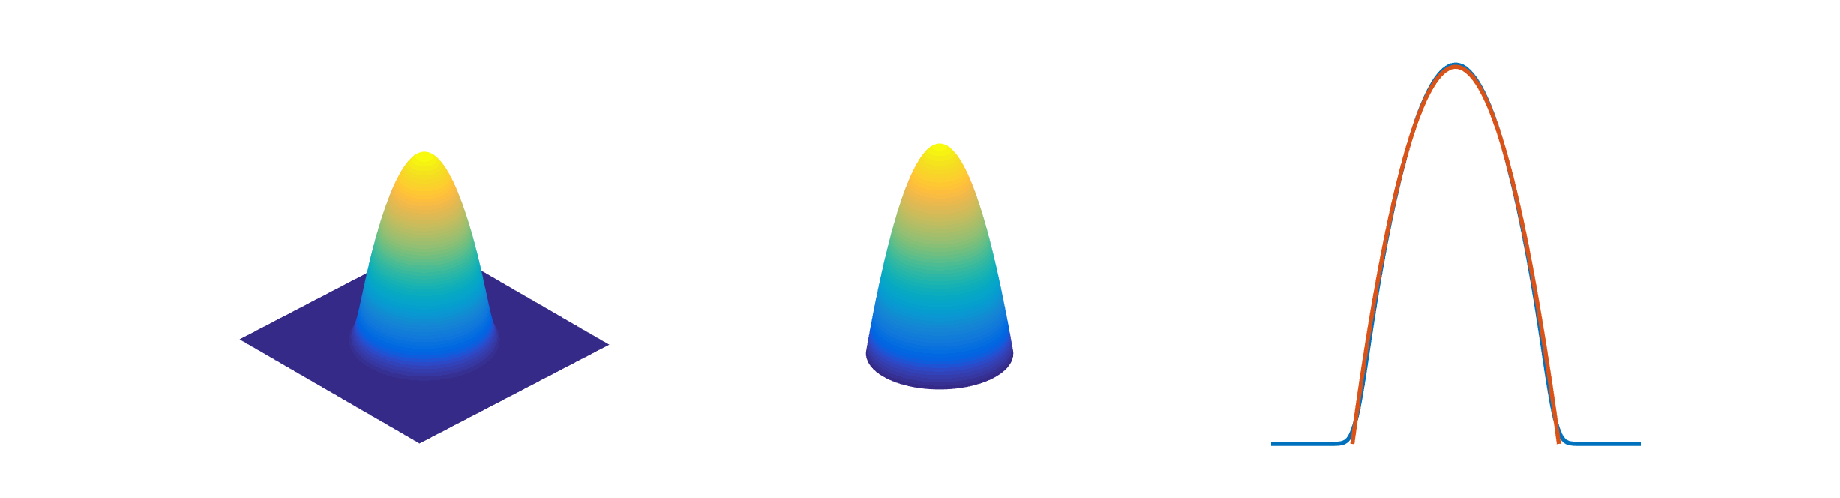
\includegraphics[width=\textwidth,trim=0ex 0ex 0ex 0ex]{Images/ch4_vtx/gpe_tf_3.pdf}
    \caption{The numerical solution (left) and Thomas-Fermi (middle) solutions for a two-dimensional condensate of $^{87}$Rb with $N=1\times 10^5$ atoms. The lineplot (right) is a central cut through both profiles showing the close match.}\label{fig:gpe_tf_3}
\end{figure}

While the Thomas--Fermi solution closely agrees with the numerical solution of the Gross--Pitaevskii equation, this solution is only applicable for stationary states with negligible kinetic energy i.e.~when the nonlinear interaction dominates over the kinetic energy term. For more complex problems involving dynamics, full numerical integration of the Gross--Pitaevskii equation is required.

One set of examples is when investigating superfluid vortex dynamics. To generate vortices in the condensate angular momentum must be added to the system. Seeding a single vortex in the condensate requires that the frequency of rotation, $\Omega$, must be higher than the critical rotation frequency $\Omega_c$, as discussed in Sec.~\ref{ss:vorticesinbec}, and in the presence of dissipation to allow for energetic losses. Numerically, this is achieved by simulating the condensate in the co-rotating frame as given by Eq.~\ref{eqn:gpe_rotation} in imaginary time, allowing for the loss of contributions from higher energy states. Experimentally, there are many ways to realise vortices in a condensate, such as stirring with a blue-detuned beam \cite{Vtx:Raman_prl_2001}, by carefully inverting the trap bias field potential \cite{Vtx:Kawaguchi_pra_2004}[Nakahara Phys. Rev. A 93, 013626], or through use of artificial gauge fields \cite{AO:Dalibard_rmp_2011}, to name but a few. In the next Sections I will concentrate on solutions where the vortices are already present in the condensate and have settled into the lowest energy configuration.


%%%%%%%%%%%%%%%%%%%%%%%%%%%%%%%%%%%%%%%%%%%%%%%%%%%%%%%%%%%%
\subsection{Few vortex condensates}
%%%%%%%%%%%%%%%%%%%%%%%%%%%%%%%%%%%%%%%%%%%%%%%%%%%%%%%%%%%%

As discussed in Section~\ref{sec:superfluid}, the discovery and manipulation of quantum vortices remains an active area of research. As the condensate kinetic energy scales as $E_k \propto l^2$ (Sec.~\ref{ss:vorticesinbec}), the system prefers to maintain singly charged vortices. In order to sustain generated vortices in a BEC the energy of the condensate with a vortex at the required rotation rate must be lower than without. For numerical solutions one method for this involves setting the rotation frequency at the required rate to support the required number of vortices.

For a single vortex in a rotating condensate in the lowest energy configuration the vortex resides at the exact centre of the trapping potential. For two vortices the radial symmetry of the system is broken, with the two vortices arranging themselves in the most favourable position to minimise their interaction energy, as with all higher states. Placing vortices of same sign into a condensate will allow them to behave as like-signed charged particles, and they will repel, and form ordered lattices with increasing vortex numbers (see Fig.~\ref{fig:few_rho}). Similarly, if instead we have the pairing of a vortex and an antivortex, they will attract, and remain in constant motion unless or annihilate for 3 or more vortex-antivortex pairings. This respective stability and dynamical behaviour can be understood by examining the velocity fields of the respective vortices, which are shown in Fig.~\ref{fig:vel_field} for like signed vortices, and Fig.~\ref{fig:vel_pm} for a vortex-antivortex pair. The velocity fields of the vortices are additive, and with same signed windings creating regions of no flow, and unlike windings creating large flows between them. The velocity field, which scales as $v_{\theta} \propto \frac{1}{r}$ becomes singular at the vortex centre, giving rise to the large field lines as observed. Fig.~\ref{fig:vel_pm_contour} shows a clearer view of the velocity fields as depicted by Fig.~\ref{fig:vel_field}, where the presence of maxima are easily observed at the cores, with field minimas observed due to the vortex-vortex interactions.

\begin{figure}\centering
    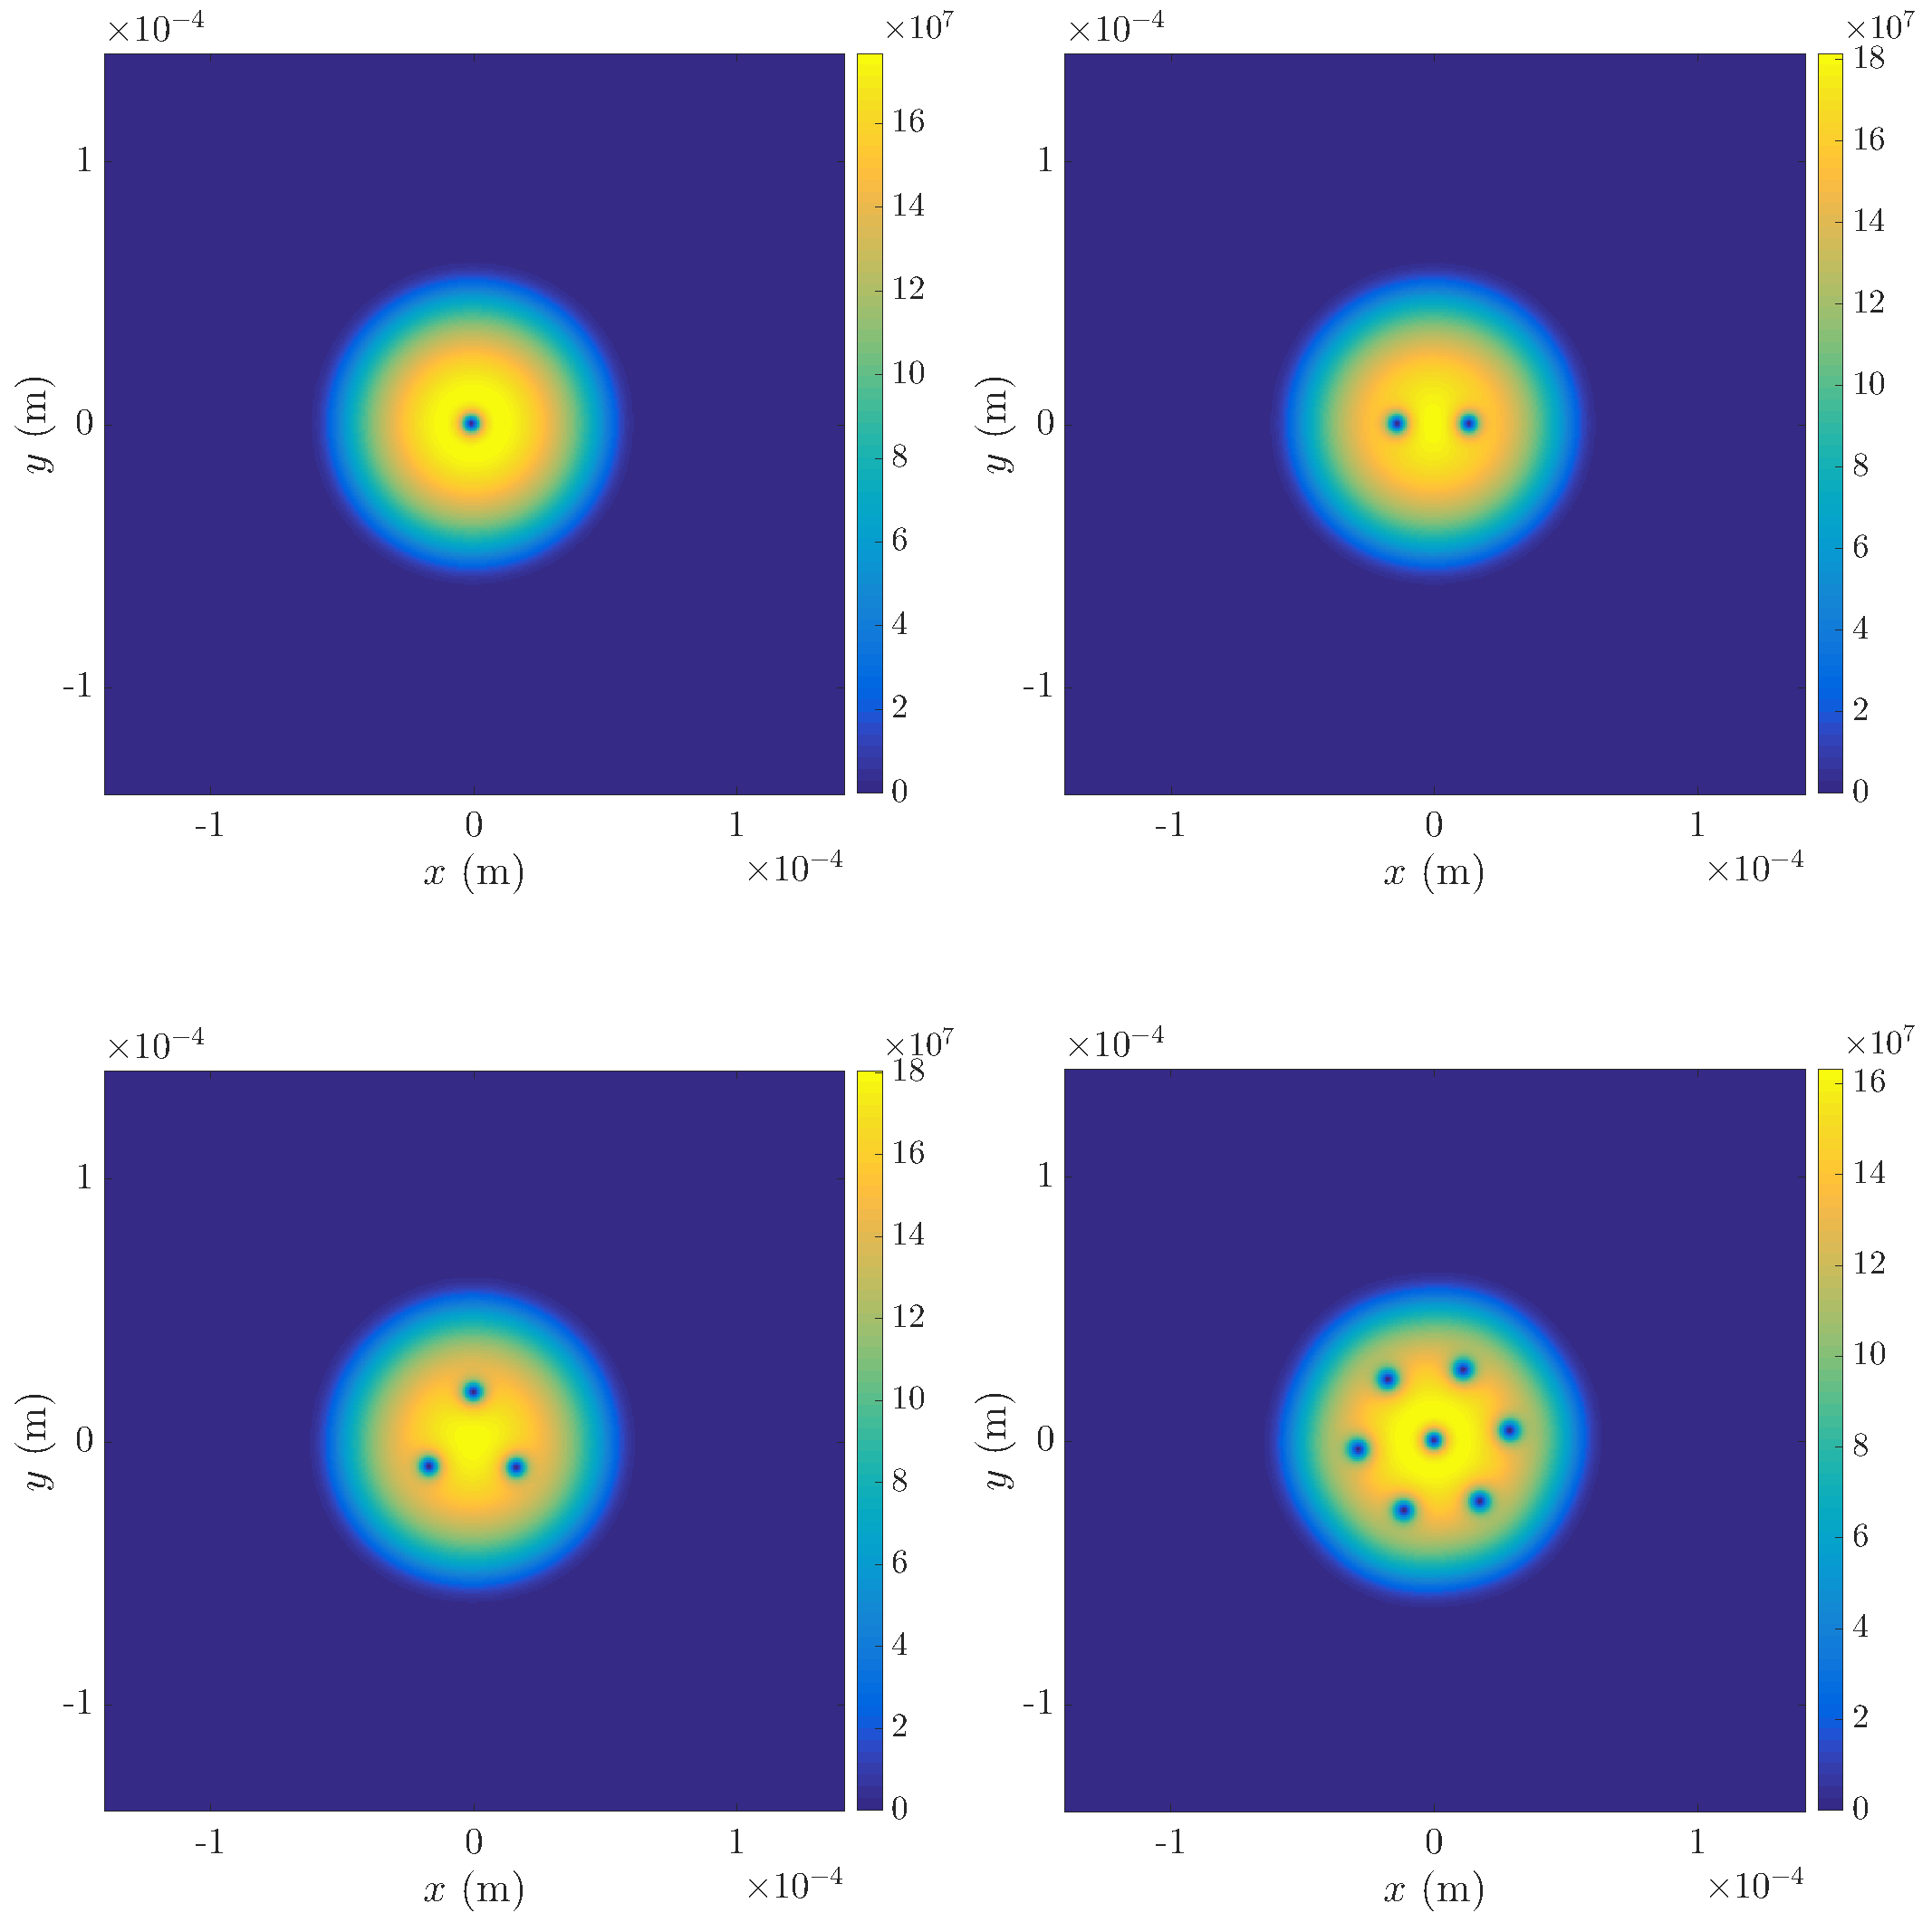
\includegraphics[width=0.48\textwidth]{Images/ch4_vtx/fewvortex_rho.pdf}
    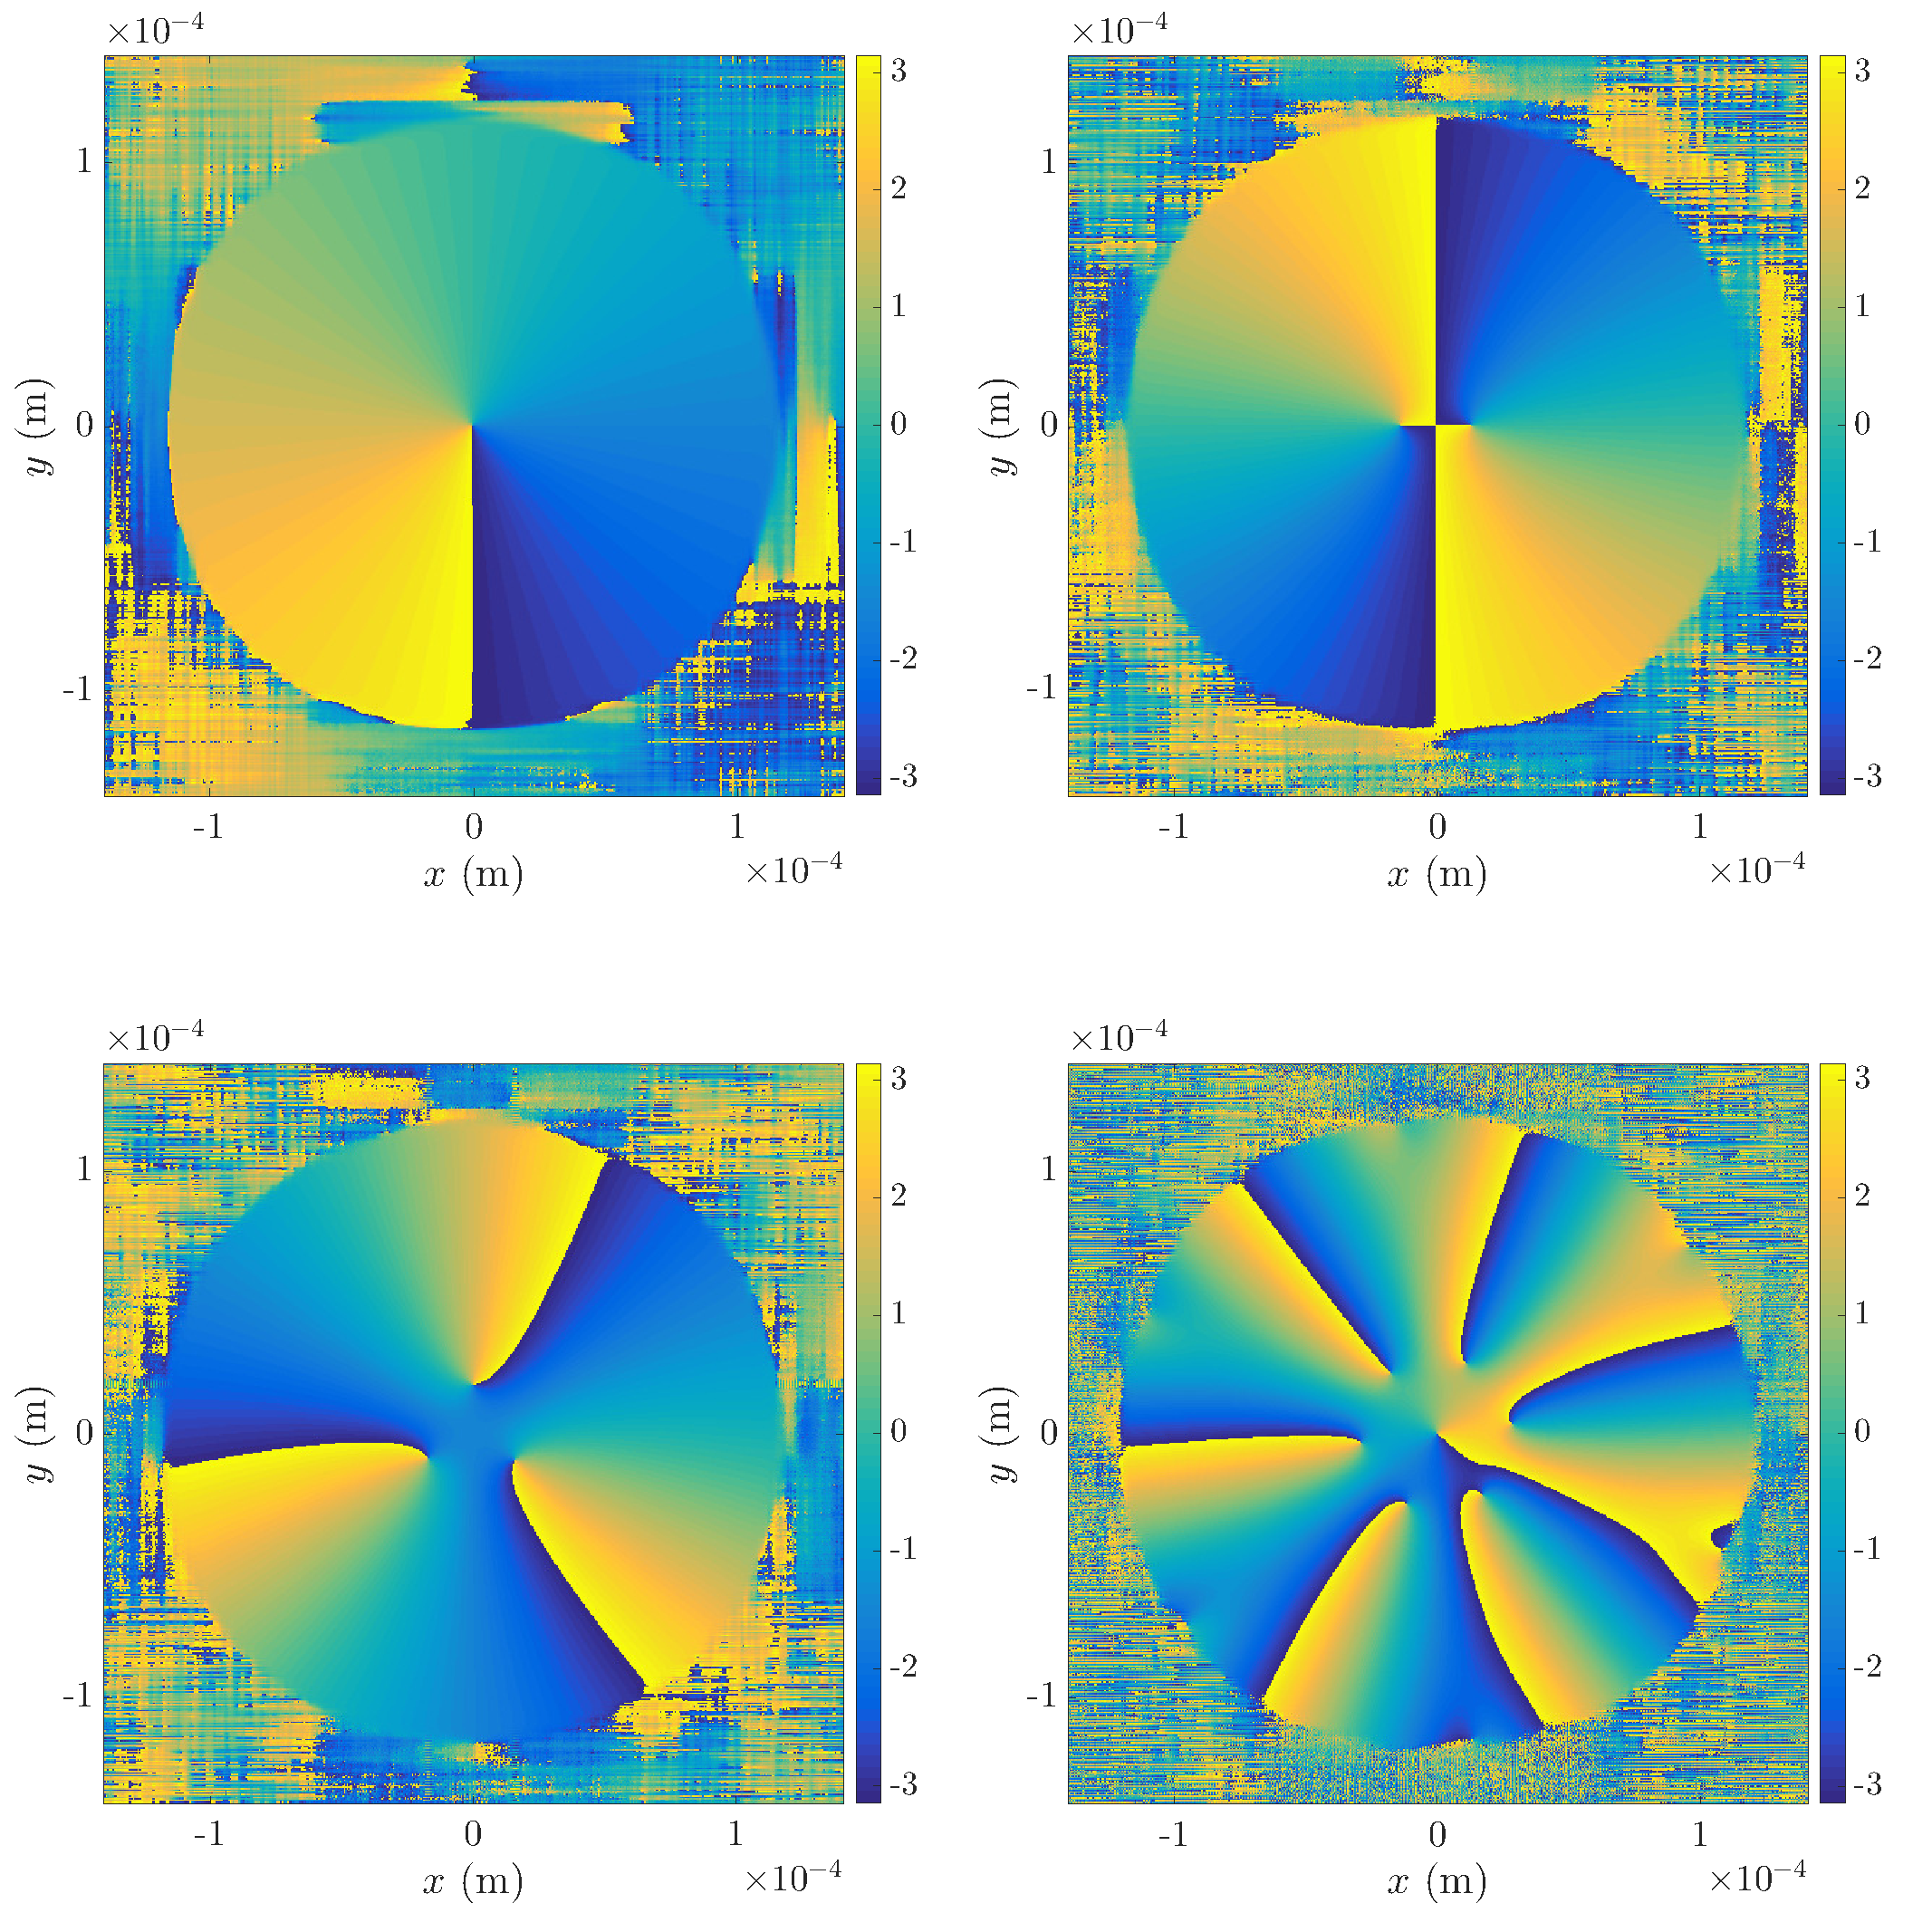
\includegraphics[width=0.48\textwidth]{Images/ch4_vtx/fewvortex_theta.pdf}
    \caption{Density (left) and phase (right) for condensates carrying 1,2,3,and 7 vortices respectively.}
    \label{fig:few_rho}
\end{figure}

\begin{figure}\centering
    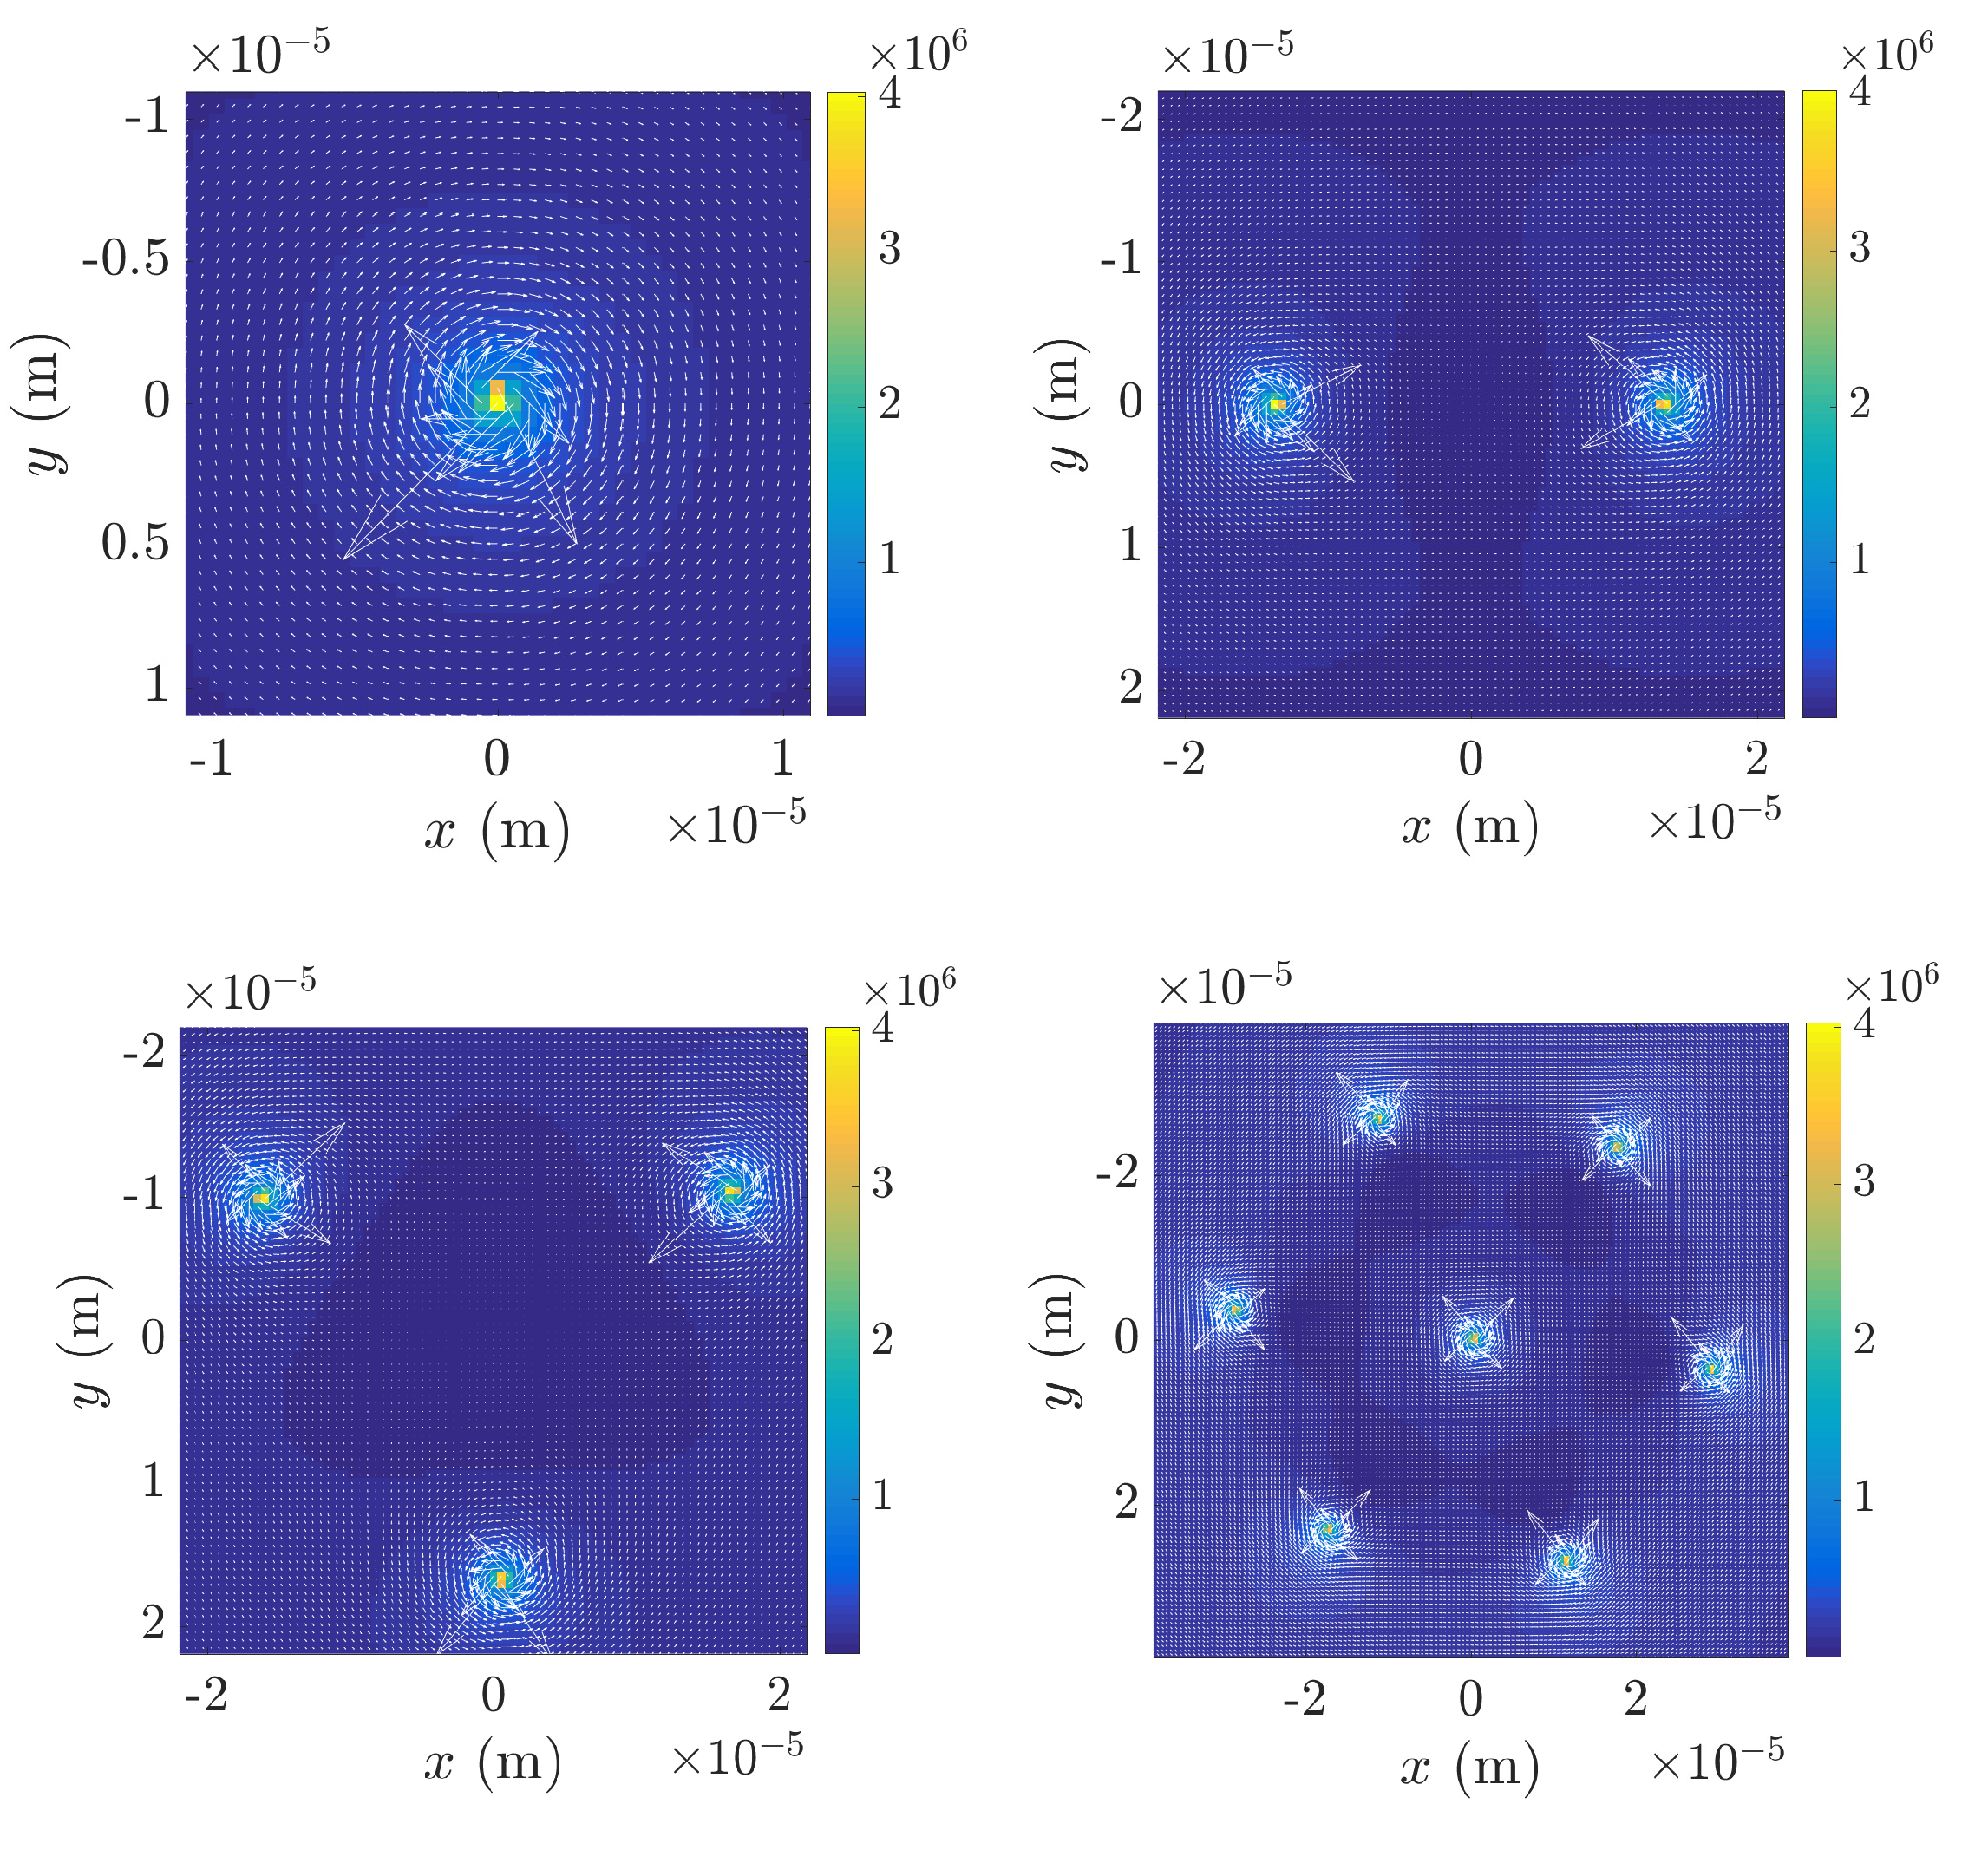
\includegraphics[width=0.95\textwidth]{Images/ch4_vtx/velocity/velocity.pdf}
    \caption{The magnitude of the velocity field and the direction of rotation of the field are indicated. The flow lines indicate the vortices are circulating clockwise. As the angular velocity becomes singular at the core centre, the flow lines grow large originating in this region.}
    \label{fig:vel_field}
\end{figure}

\begin{figure}\centering
    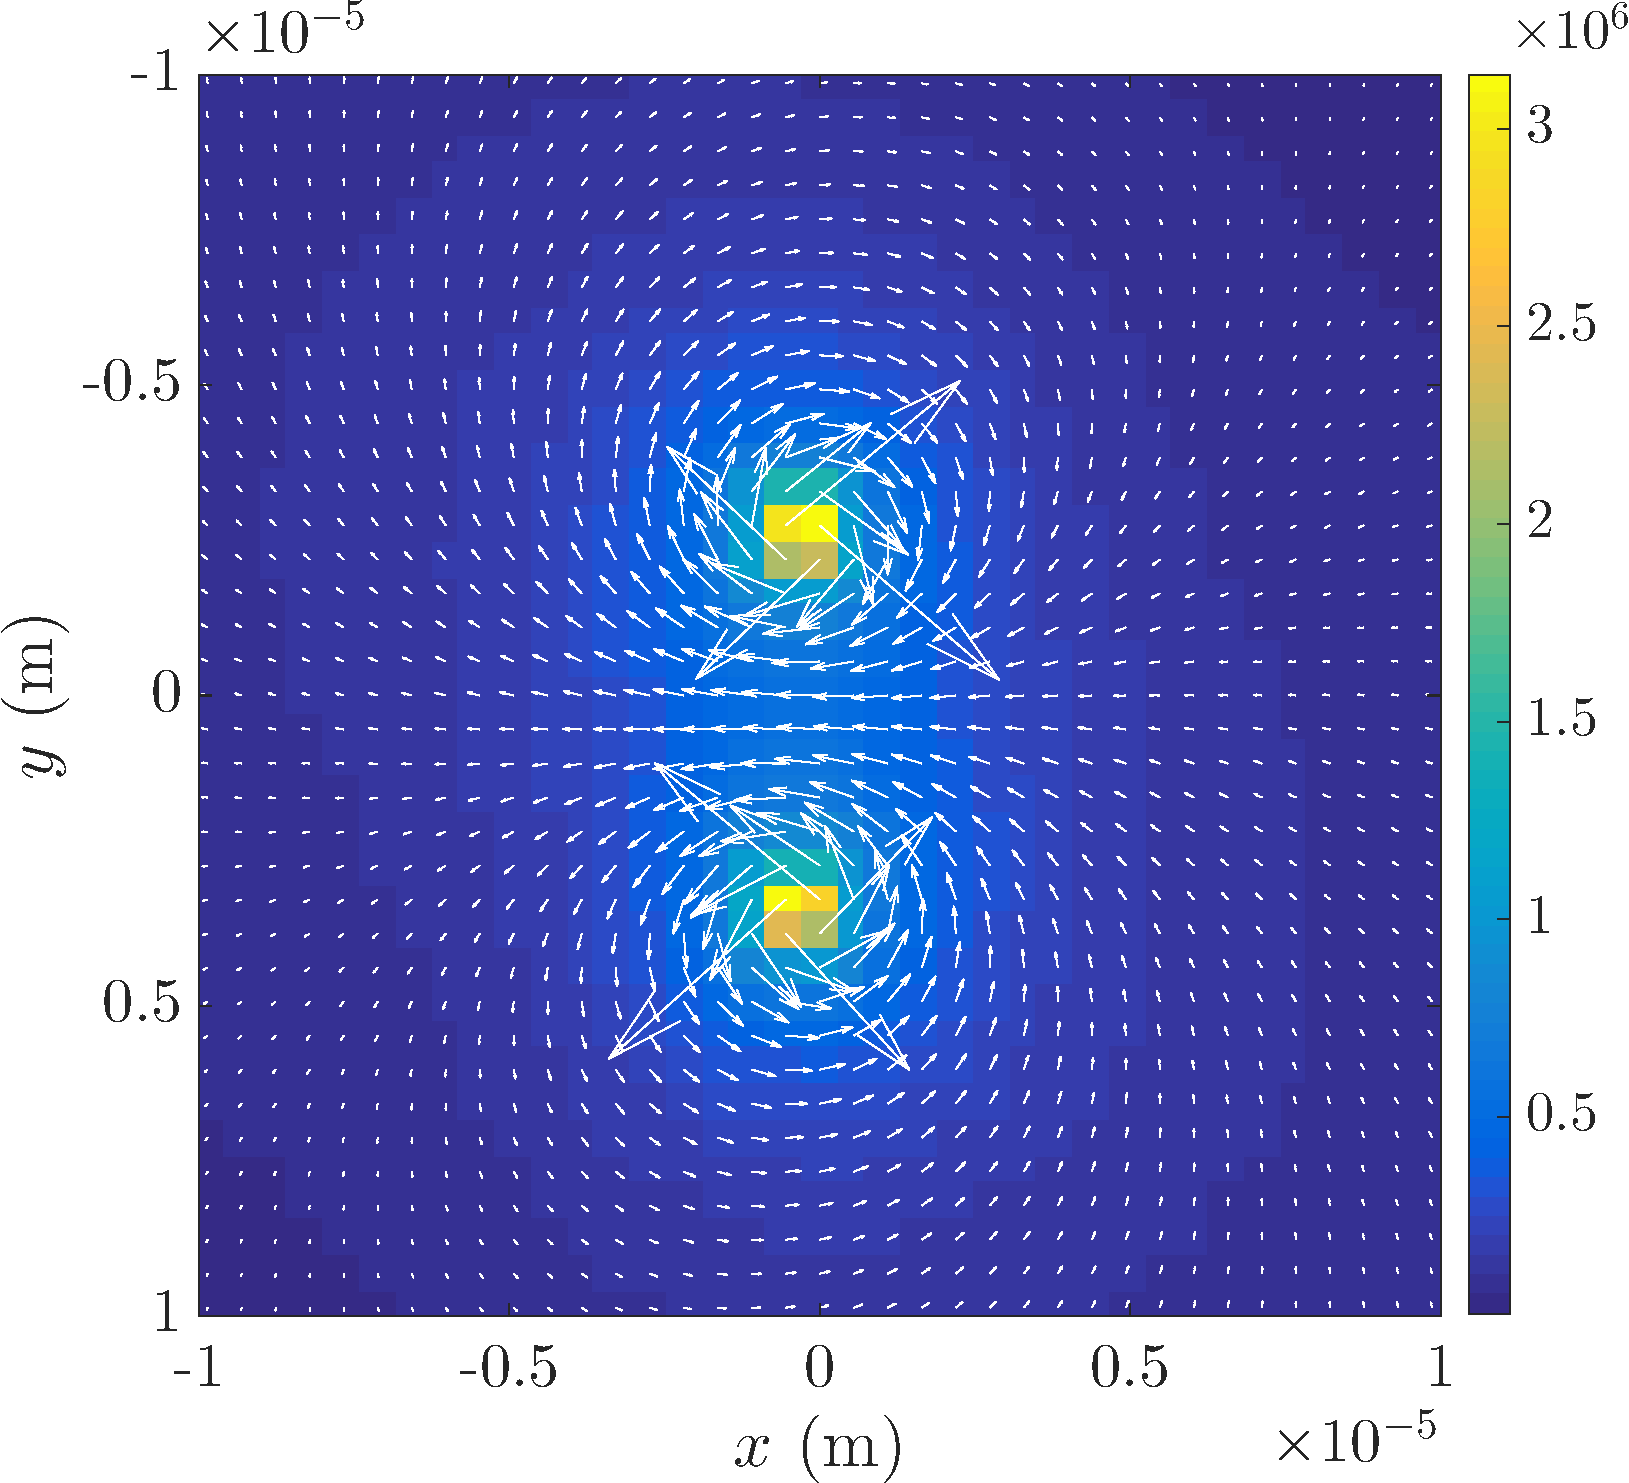
\includegraphics[width=0.45\textwidth]{Images/ch4_vtx/velocity/vtx_antivtx_vel}
    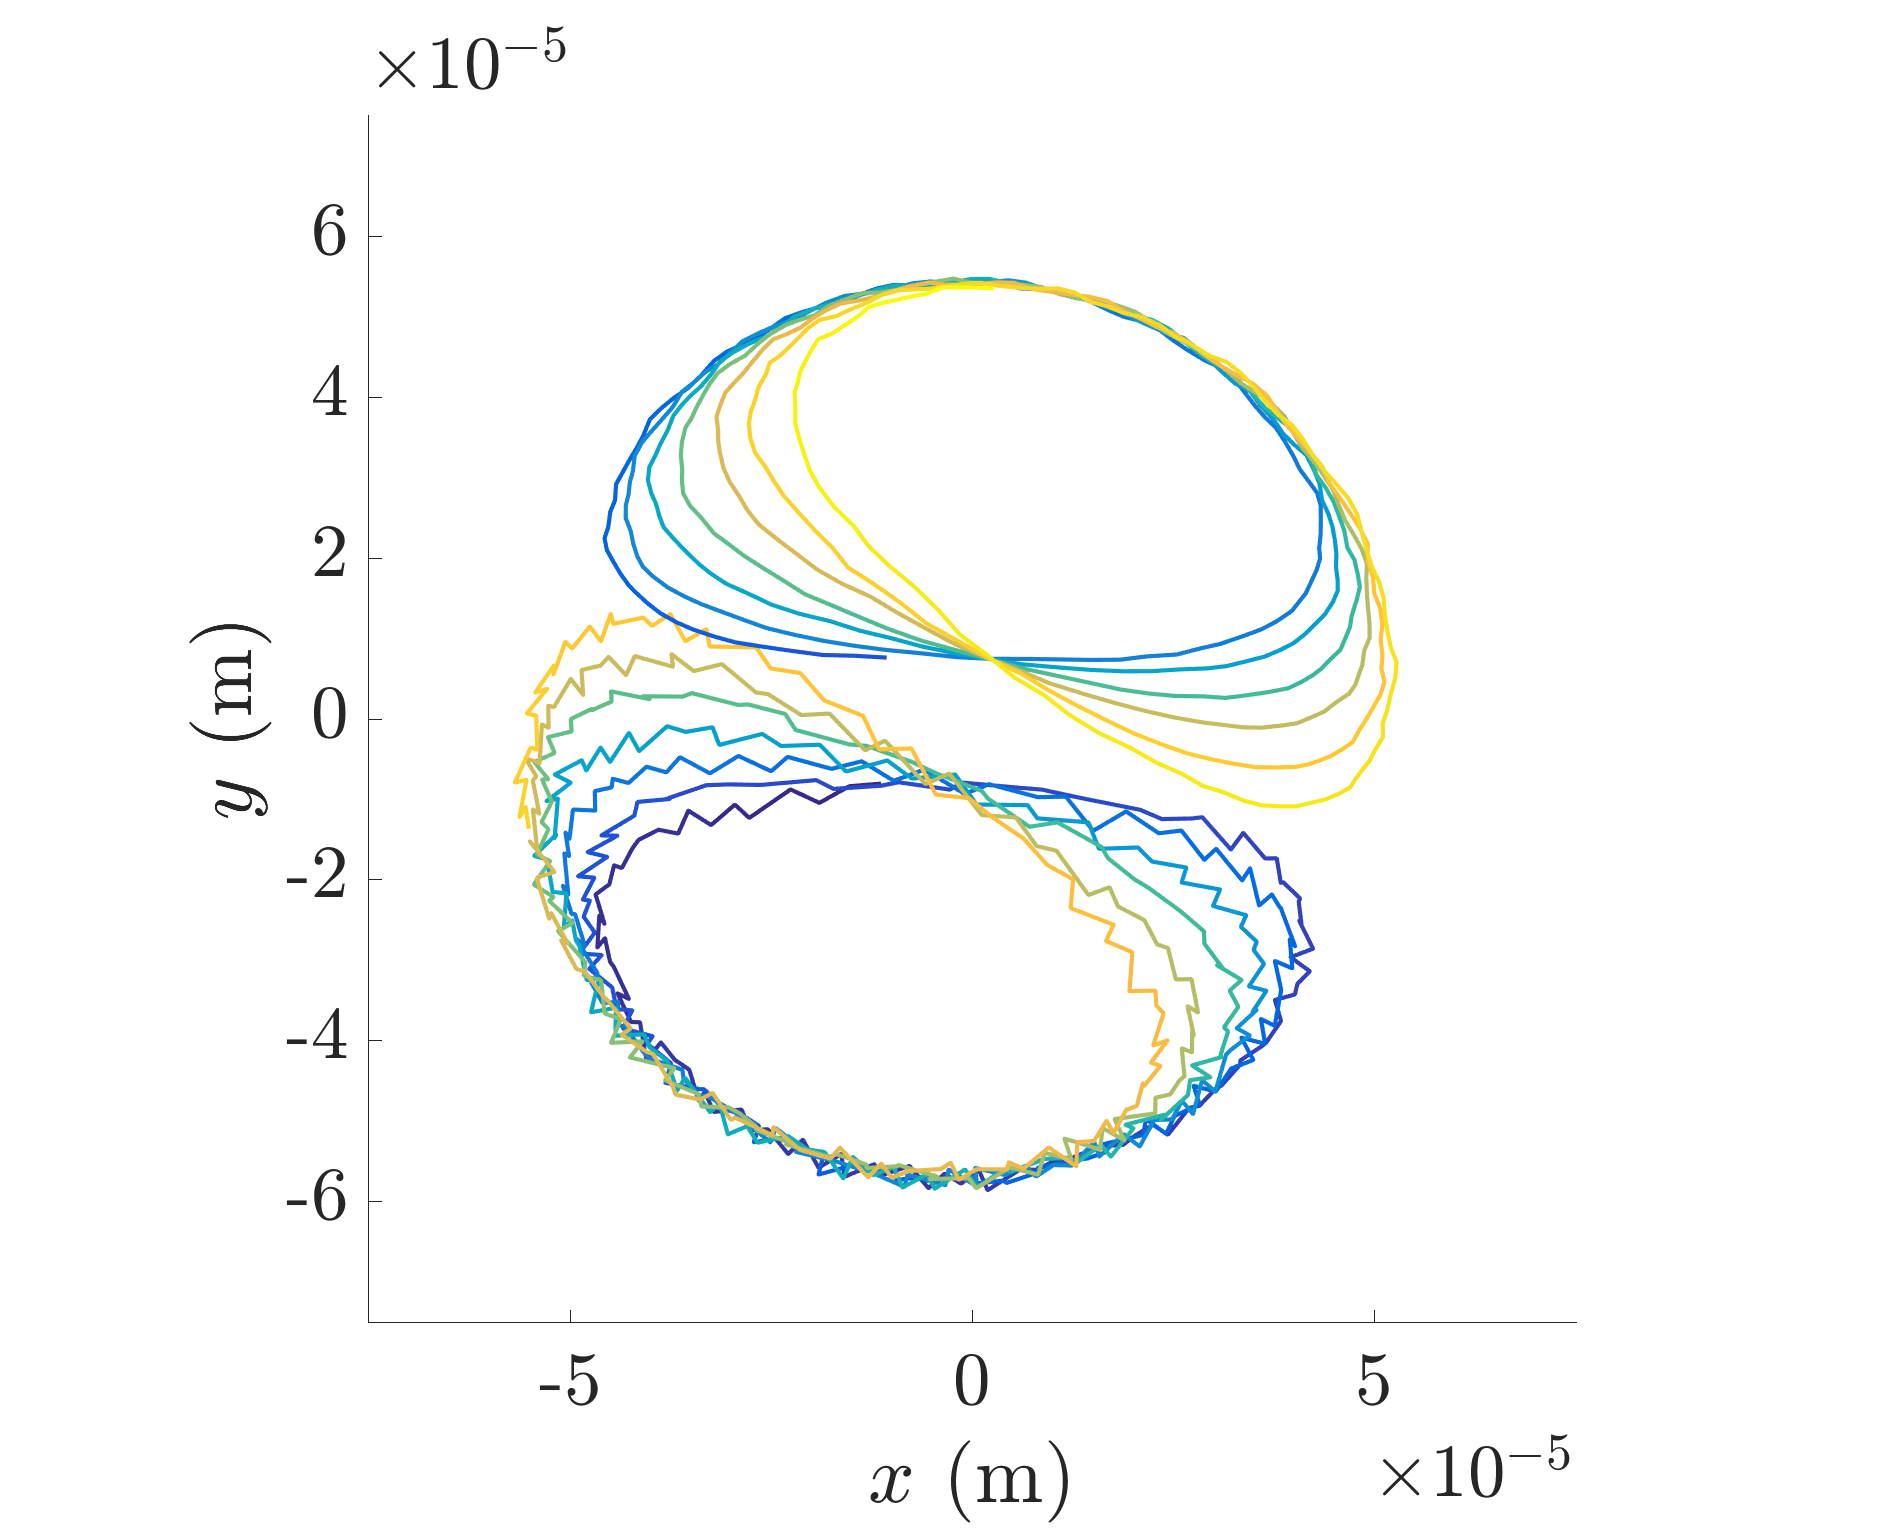
\includegraphics[width=0.45\textwidth]{Images/ch4_vtx/vtx_antivtx_traj}
    \caption{(Left) Velocity field originating from vortex and antivortex present in a condensate. (Right) Trajectories of vortex and antivortex in a condensate in the lab frame. Vortices travel on circulating paths which will always intersect through their starting position. Color is used to represent the same times for both vortex and antivortex, which is on the order of seconds.}
    \label{fig:vel_pm}
\end{figure}

\begin{figure}\centering
    \includegraphics[width=0.95\textwidth]{Images/ch4_vtx/velocity/vel_axis_png}
    \caption{The magnitude of the velocity field for small numbers of vortices in a condensate. The velocity field can be seen to become singular at the centre. Regions of minimal velocity are seen, wherein the opposing field lines negate one another.}
    \label{fig:vel_pm_contour}
\end{figure}


%%%%%%%%%%%%%%%%%%%%%%%%%%%%%%%%%%%%%%%%%%%%%%%%%%%%%%%%%%%%
\section{Rapidly rotating vortex lattice}
%%%%%%%%%%%%%%%%%%%%%%%%%%%%%%%%%%%%%%%%%%%%%%%%%%%%%%%%%%%%

%%%%%%%%%%%%%%%%%%%%%%%%%%%%%%%%%%%%%%%%%%%%%%%%%%%%%%%%%%%%
\subsection{Model system}\label{sec:modelsystem}
%%%%%%%%%%%%%%%%%%%%%%%%%%%%%%%%%%%%%%%%%%%%%%%%%%%%%%%%%%%%

For the body of work to follow I will assume that the trapping frequency along the $z$-axis, $\omega_z$, is much larger than the one along the transverse axis, $\omega_\perp$. This allows the condensate to be modeled as a quasi-2d pancake-shaped geometry, and as discussed earlier is a valid assumption for realistic experimental systems~\cite{BEC:Fetter_revmodphys_2009}. Integrating along the $z$ dimension ($\textbf{r}\equiv [x,y]$) simplifies the analysis of the system and resulting dynamics, which are capably described in two-dimensions. I assume the standard formalism of a single component Bose--Einstein condensate in a radially symmetric trap of frequency $\omega_\perp = 2\pi \times 1$ Hz. By tightly confining the condensate along the $z$-dimension, with trapping frequency $\omega_z = 2\pi\times 16$ Hz, such that $\omega_z \gg \omega_\perp$, the condensate enters the pancake-shaped geometry. As the energy required to excite any higher modes along $z$ is $\geq \hbar\omega_z$, one can assume all excitations are planar along the radial coordinate $x-y$ axes, with the $z$ axis in the harmonic oscillator ground state. Modeling of this system is performed in the mean-field limit, given by the Gross--Pitaevskii equation, with Hamiltonian


\begin{equation}\label{eqn:gpe_h0}
	H_{\mathrm{GP}} = -\frac{\hbar^2}{2m}\nabla^2 + \frac{1}{2}m\omega_{\perp}^2\mathbf{r}^2 + g\vert\Psi(\mathbf{r},t)\vert^2.
\end{equation}

Here $g$ describes the interaction between atoms in the condensate, given by \begin{equation}
g = \frac{4\pi\hbar^2a_s}{m},
\end{equation}
where $a_s$ is the s-wave scattering length of the atomic species. Restricting the system to a two-dimensional geometry also requires the move to an effective interaction which encompasses the net effect of the $z$-dimension. This is enabled by scaling the interaction by the length of the harmonic oscillator along the $z$-dimension~\cite[pg. 456]{BK:Pethick_smith_}, and for the given parameters becomes
\begin{equation}
g_{2D} = g\sqrt{\frac{m\omega_z}{2\pi\hbar}} = 4g \sqrt{\frac{m}{\hbar}}.
\end{equation}

To describe the system we enter the co-rotating, which is done by adding the angular momentum operator to the Hamiltonian. The time dependent dynamics of the system can be analysed using the GPE form as given by eq.~\ref{eqn:gpe2d}
\begin{equation}\label{eqn:gpe2d}
	i\hbar\frac{\partial}{\partial t}\Psi(\mathbf{r},t) = \left[ H_{\text{GP}}  -  \Omega_z L_z \right] \Psi(\mathbf{r},t),
\end{equation}

This is the form of \ref{eqn:gpe} for a two-dimensional harmonically trapped condensate. If the angular rotation frequency approaches the condensate trapping frequency, $\Omega_z \approx \omega_\perp$ the condensate gains a large triangular lattice of vortices.  The effect of setting $\Omega=\omega_\perp$, can be partially understood in a mean field setting by rewriting the GPE in the form
\begin{equation}
    i\hbar\partial_t \Psi =
    \left(\frac{1}{2m}(-i\hbar\nabla - m\Omega\times\mathbf{r})^2 + \frac{m}{2}(\omega_\perp - \Omega)^2{r}^2 + g_{2d}|\Psi|^2 \right)\Psi.
\end{equation}
The above Hamiltonian rises from the equivalence between a rotating condensate and that of a non-relativistic charged particle in a magnetic field, described by the Hamiltonian
\begin{equation}
     H_L = \frac{1}{2m}\left(-i\hbar \nabla  - q\mathbf{A}\right)^2 + q\phi
\end{equation}
where $q$ is the particle charge, $\mathbf{A}$ is the respective gauge potential, and $\phi$ the respective scalar potential. One can see that were the rotation and trapping frequencies equal, the condensate would no longer see a confining potential, due to the centrifugal forces experienced, given by the term $-m\Omega^2r^2/2$, resulting in an untrapped system.

As $\Omega$ approaches $\omega_\perp$ the use of mean-field theory becomes less effective, as the system enters a strongly correlated regime. This is often
characterised by the filling factor (or filling fraction) $\nu=N/N_v$, i.e.~the ratio of atoms to vortices discussed in Sec.~\ref{sec:intro}. Values of $10 \leq \nu \leq 1000$ enter the so-called ``mean-field quantum Hall'' regime, with Gross--Pitaevskii theory working well. For values $\nu \leq 10$ the system is said to be strongly correlated~\ref{BEC:Fetter_revmodphys_2009}, and will require the use of a discrete boson model, which becomes next to impossible for a realistic number of atoms in a condensate. Assuming an upper limit frequency of $\Omega = 0.995\omega_\perp$ allows the system to have a very large vortex lattice, and still be described capably by mean-field theory \cite{Vtx:Fetter_rmp_2009}.

For this work eq.~\eqref{eqn:gpe2d} will be numerically solved, using the pseudospectral Fourier split operator method making use of GPU computing~\cite{sec:GPUE}. For realistic experimental parameters I assumed  $N=9.8\times 10^5$ atoms of $^{87}$Rb, with an s-wave scattering length of $a_s=4.76\times10^{-9}$ m~\cite{AO:Roberts_prl_1998}. The numerically evaluated ground-state for the given set of parameters is previously shown in Fig.~\ref{fig:showingoff} with a radius of approximately $3.5\times 10^{-4}$ m, though solutions were also obtained for lower resolutions and different maximum system sizes.

For the chosen parameters, the number of vortices within the visible density region is approximately 600, giving a filling factor of $\nu \approx 800 $. This places the system within the mean-field quantum Hall regime, and therefore a description using Gross--Pitaevskii theory is adequate~\cite{Vtx:Schweikhard_prl_2004}.

To numerically solve for this system, I used GPUE, assuming an initial wavefunction guess of a two-dimensional gaussian having some finite overlap with the groundstate of the system in the absence of angular rotation. Following an imaginary time-evolution as outlined in Sec.~\ref{sec:numerics}, the groundstate of the condensate in a harmonic potential was found. Starting with a condensate without vortices, I linearly ramp the rotation frequency, as to avoid the disordering issue as discussed in Sec.~\ref{ss:ang_mom_fso}. For a ramp of the rotation frequency during imaginary time evolution, I essentially follow the groundstate solution at all times. This has an added advantage of returning a groundstate solution for any required rotation frequency, with the number of vortices increasing for higher frequencies. An example of several states from a single simulation are given in Fig.~\ref{fig:inc_omega}. The previously discussed resolution considerations become apparent as the rotation rate is increased for both position and momentum space representations of the wavefunction. A sample movie of the generation is available here~[goo.gl/30Mj1q]\cite{goo.gl/30Mj1q}, wherein I ramp the frequency from $\Omega/\omega_\perp = 0.39 \to 0.995$ and plot the wavefunction density $|\Psi(\mathbf{r},t)|^2$. It can be noted however that as higher rotation frequencies are reached, the rate at which vortices enter the condensate increases. It can also be observed that with a well ordered lattice in the central region, this has little to no effect to incoming vortices, which arrange themselves into the expected lattice positions.

\begin{figure}\centering
    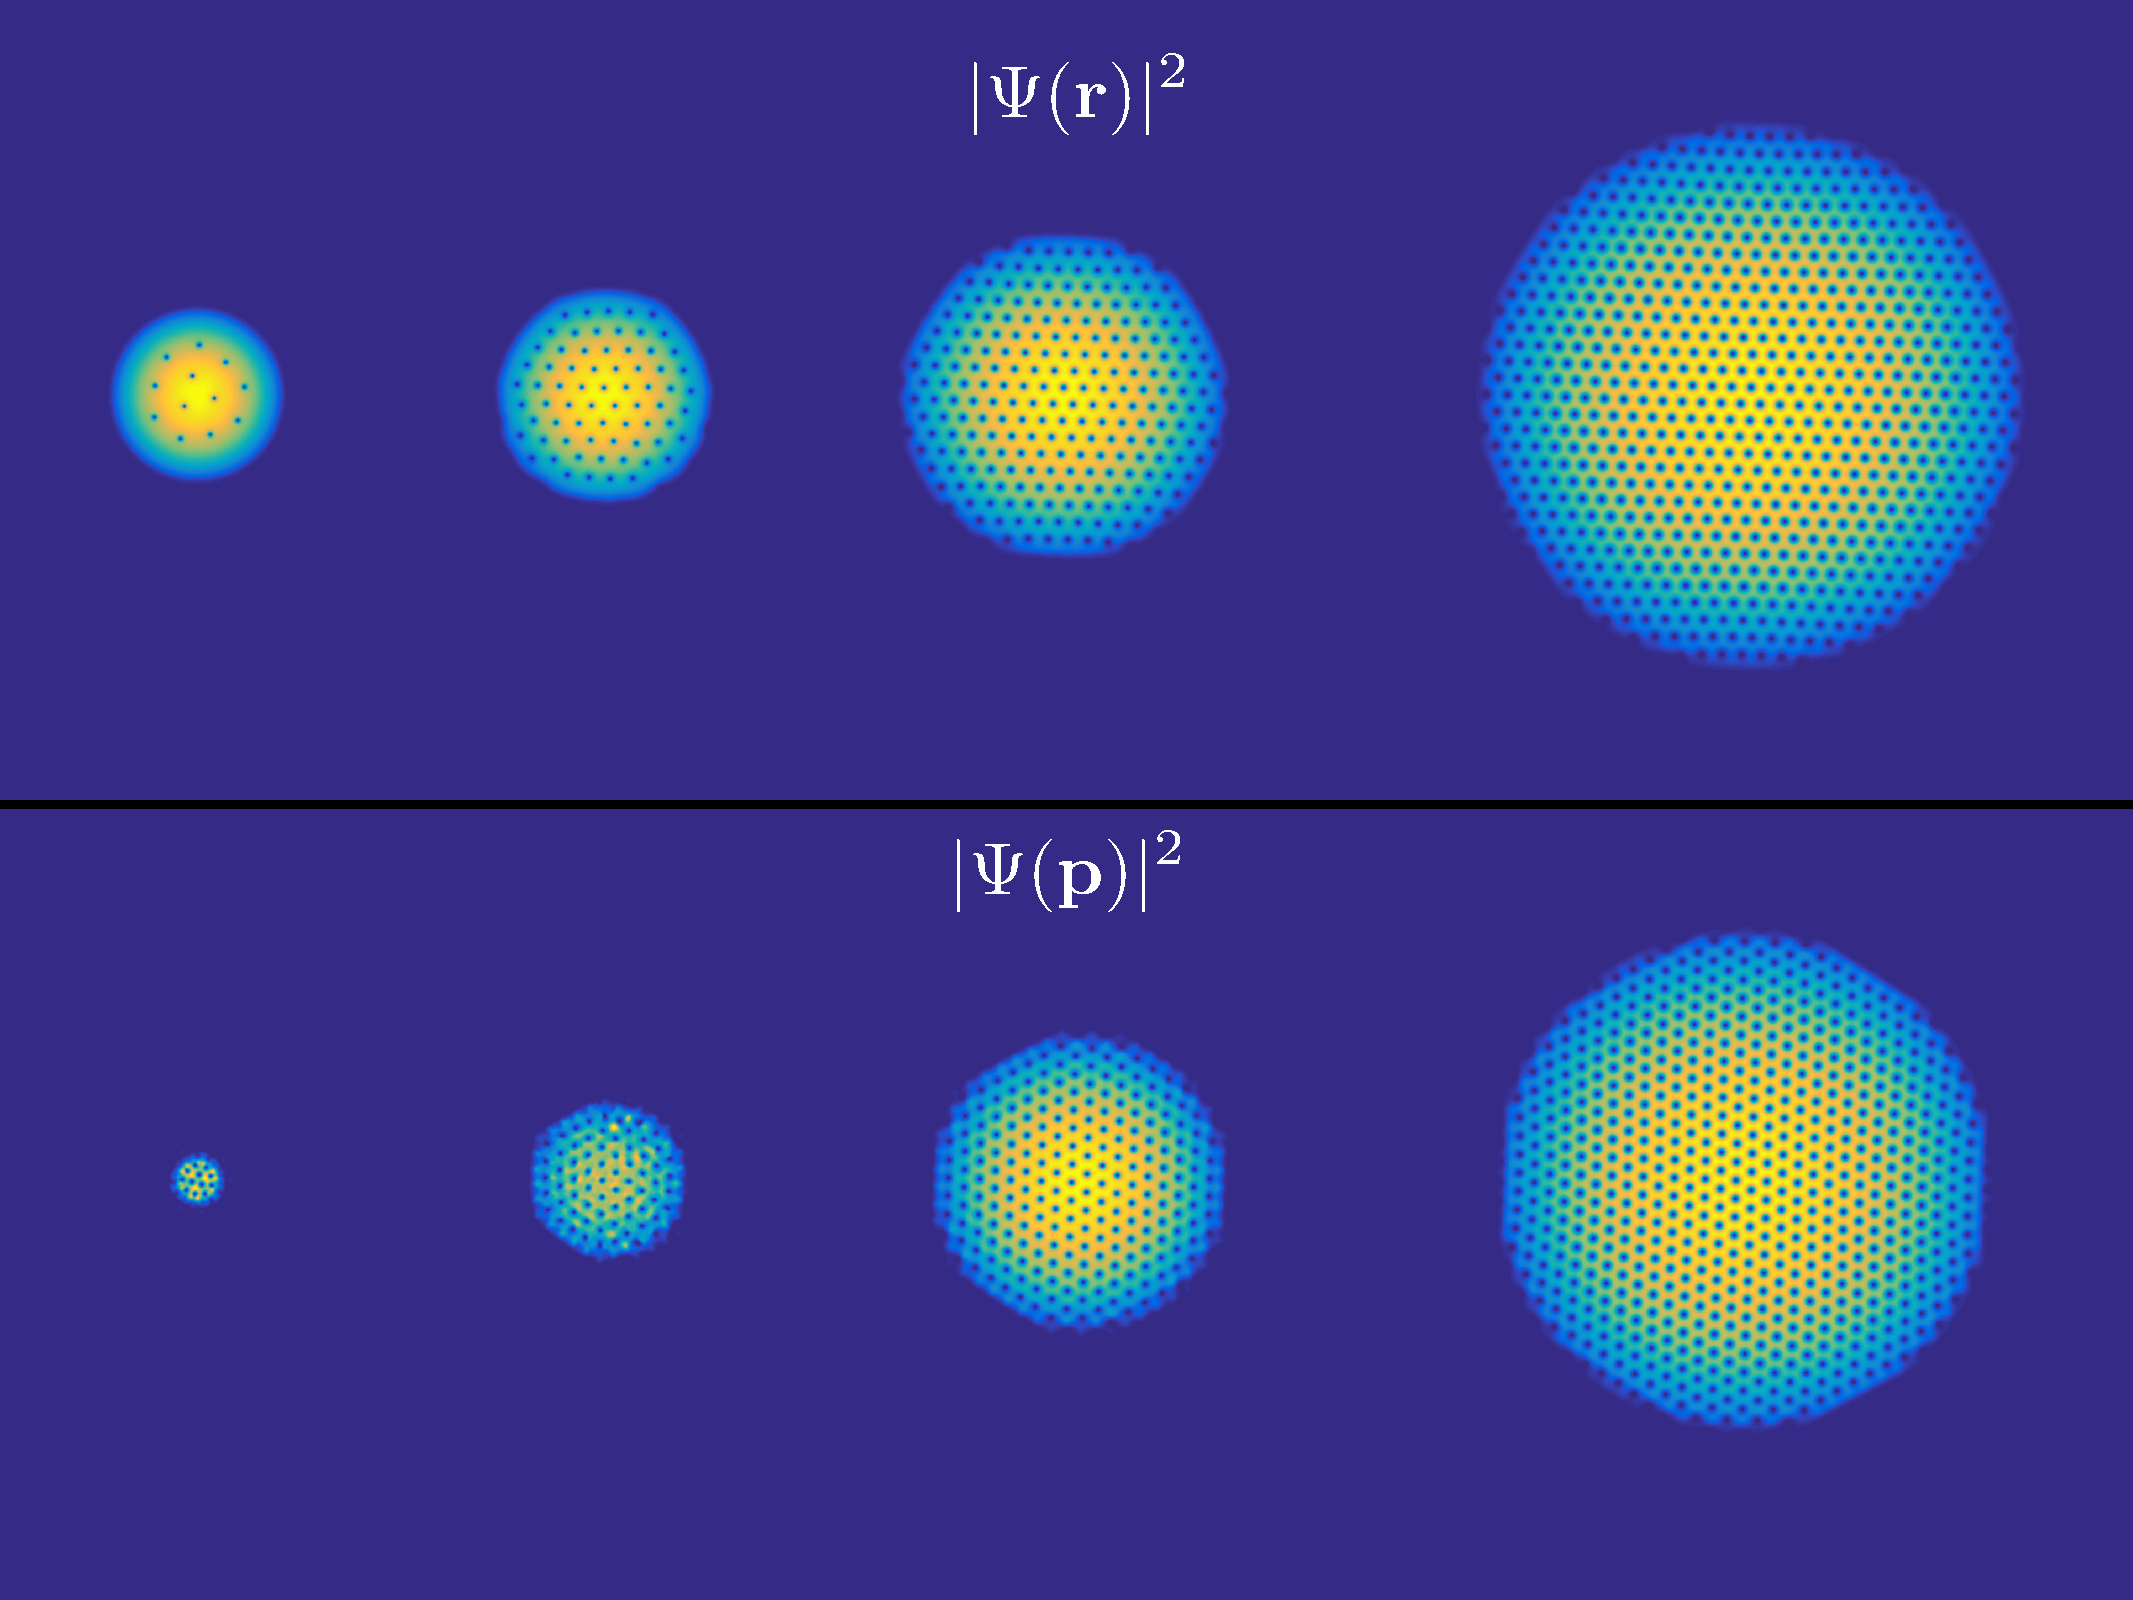
\includegraphics[width=0.85\textwidth]{Images/ch4_vtx/ramp_omega.pdf}
    \caption{The density distributions of the wavefunction in position (top) and momentum (bottom) space are given for rotation frequencies (L-R) $\Omega/\omega_\perp=[0.366,0.796,0.962,0.995]$. The color axis differs for each plot, as a constant axis is difficult to view densities across all magnitudes. The growth rate of the condensate radius in both position and momentum space becomes large when $\Omega \approx \omega_\perp$.}
    \label{fig:inc_omega}
\end{figure}

If the linear ramp is performed too quickly, or if I instantaneously choose a groundstate with a large amount of angular momentum, the vortices tend to enter from the boundary all at one instance, and fail to ever find a well ordered groundstate. An example of this such issue is given by Fig.~\ref{fig:malformed_lattice}, and indicates the need for a slow ramp of $\Omega$ that is essentially adiabatic in imaginary time.

\begin{figure}
    \centering
    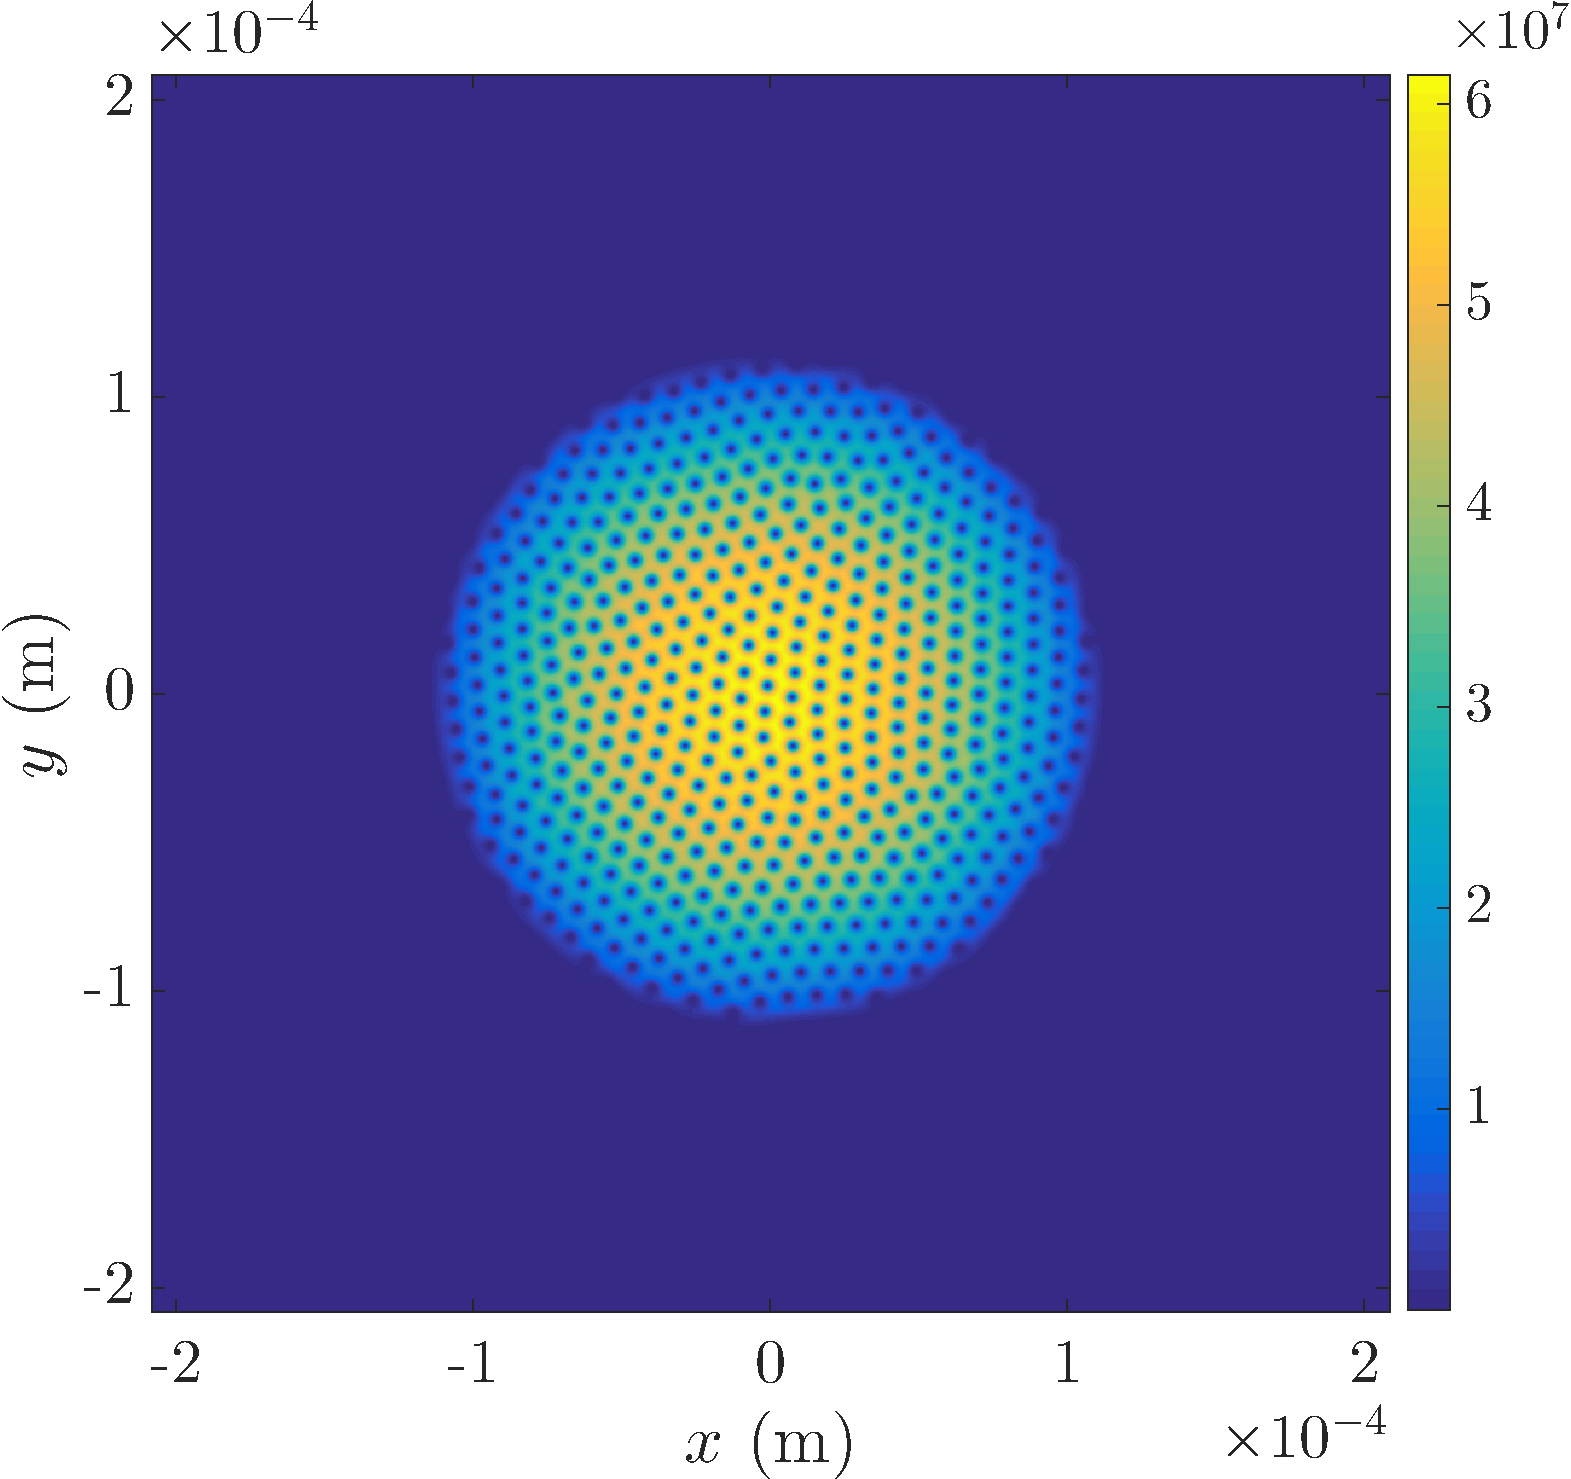
\includegraphics[width=0.65\textwidth]{Images/ch4_vtx/toofast_099_1e7}
    \caption{Disordered lattice resulting from starting in imaginary time evolution at the required rotation rate (here $\Omega=0.99\omega_\perp$). If the rotation frequency is chosen too large without allowing the lattice to form and order, the resulting vortices all enter instantaneously and compete for position. }
    \label{fig:malformed_lattice}
\end{figure}

The velocity field direction and magnitude of the rapidly rotating vortex lattice is is known to exhibit solid-body-like rotation. This can be observed in Fig.~\ref{fig:solidbody}, where the coarse-grained flow of the velocity field increases as a function of the distance from the lattice centre. This rigid-body behaviour allows us to assume and treat the lattice as a solid object. One can investigate the overall effect of perturbations to both global condensate order, and local to individual vortices.
\begin{figure}\centering
    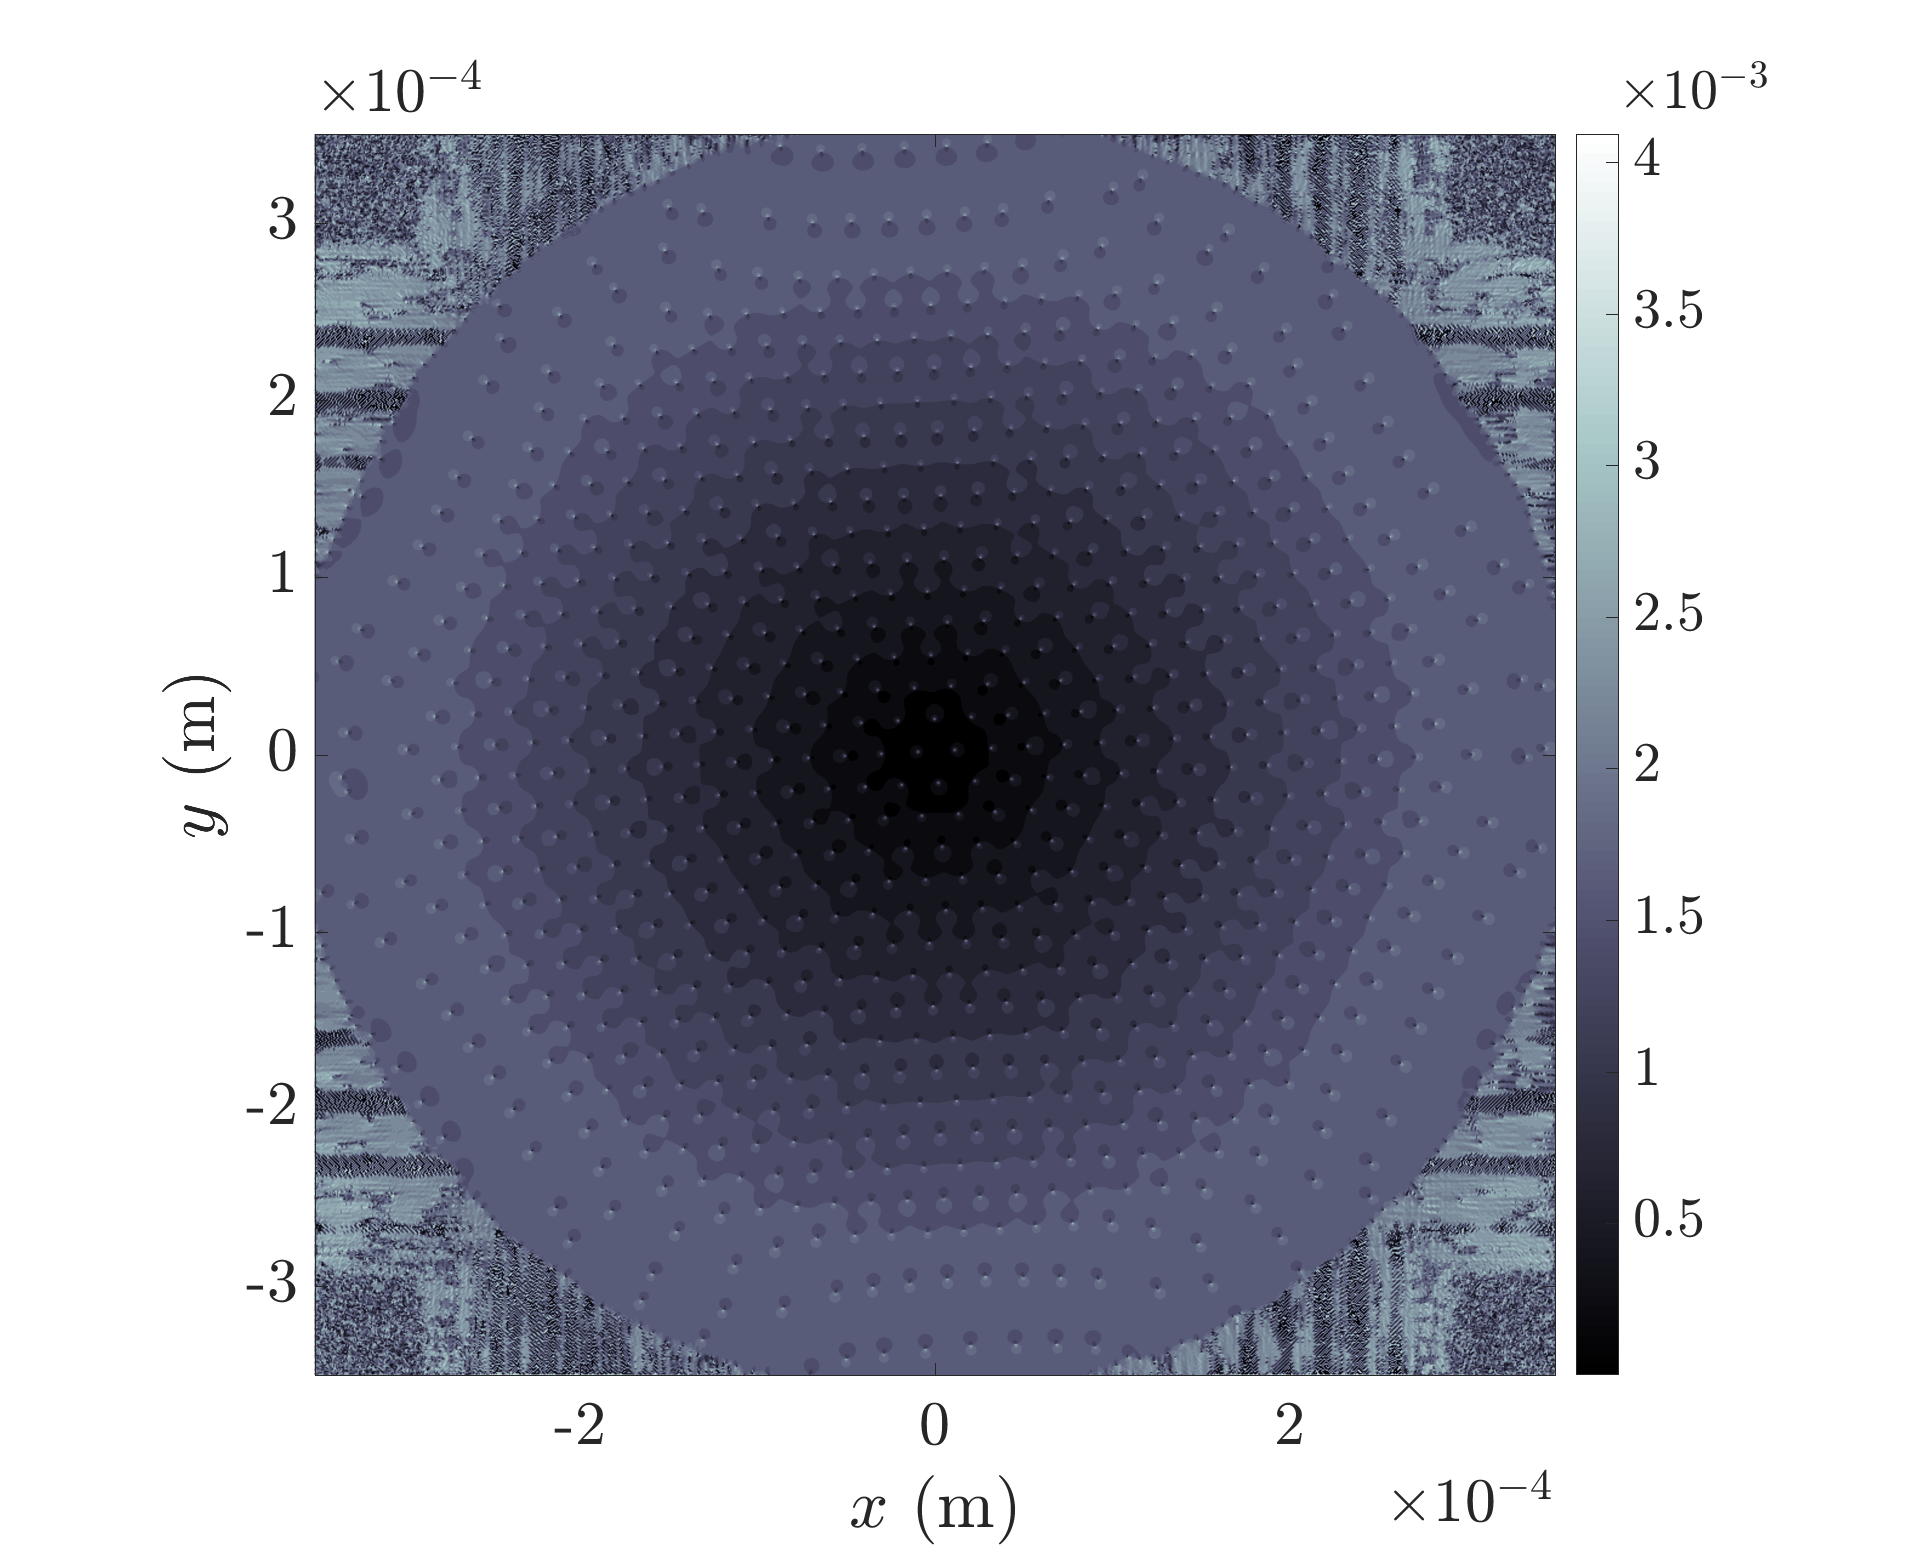
\includegraphics[width=0.85\textwidth,clip,trim={0cm 2cm 0 2cm}]{Images/ch4_vtx/velocity/solidbody}
    \caption{Magnitude and direction of flow of the velocity field for the vortex lattice in the rapidly rotating frame. The almost solid-body like behaviour can be seen, where the coarse-grained condensate velocity increases as a function of distance from the centre. Close to the vortex cores the fields retain their $1/r$ profile, becoming singular at the core centres.}
    \label{fig:solidbody}
\end{figure}

%%%%%%%%%%%%%%%%%%%%%%%%%%%%%%%%%%%%%%%%%%%%%%%%%%%%%%%%%%%% 1
\section{Condensate perturbations}
%%%%%%%%%%%%%%%%%%%%%%%%%%%%%%%%%%%%%%%%%%%%%%%%%%%%%%%%%%%%
%%%%%%%%%%%%%%%%%%%%%%%%%%%%%%%%%%%%%%%%%%%%%%%%%%%%%%%%%%%% a
\subsection{Trapping potential control}\label{ss:pert_opt_latt}
%%%%%%%%%%%%%%%%%%%%%%%%%%%%%%%%%%%%%%%%%%%%%%%%%%%%%%%%%%%%
With the model system outlined in Sec.~\ref{sec:modelsystem}, let us now imagine an abrupt change to this Hamiltonian, such that, $H = H_{\textrm{GP}} + f(t) V_{\textrm{ext}}$, where  $V_{\textrm{ext}}$ is an arbitrary external potential, and $f(t)$ is some function of time to control the application of $V_{\textrm{ext}}$ . In this scenario, the wavefunction, formerly a stationary state of $H_{\textrm{GP}}$, will no longer remain so in the new Hamiltonian provided that $H_{\textrm{GP}} $ and $f(t) V_{\textrm{ext}}$ are non-commuting. Any modification of the Hamiltonian in this way can be viewed as a method for changing the phase of the resulting wavefunction, assuming the time of application of the additional term is much shorter than the timescale of condensate dynamics.
%\begin{equation}
%    e^{i\phi} \mapsto \exp\left(-i\frac{Ht}{\hbar}\right),
%\end{equation}
The resulting form of the evolution operator can be given as
\begin{subequations}
\begin{align}
    \Psi_0 &= |\Psi_0|e^{i\theta_0} \\
    \Psi(t) &= \Psi_0 e^{-\frac{i H t}{\hbar}} \\
            &= |\Psi_0| e^{i\left(\theta_0 - \frac{H t}{\hbar}\right)} \nonumber \\
    \theta^{'} &= \theta_0 - \frac{H t}{\hbar}
\end{align}
\end{subequations}
wherein I have made use of Eq.~\ref{eqn:madelung}. By modifying the Hamiltonian the resulting components of the wavefunction see a different phase which governs their evolution. One commonly used method to manipulate the Hamiltonian is through the use of optical potentials, which offer large degrees of control over the respective Hamiltonian \cite{Many-body physics with ultracold gases}. An arbitrary optical field, described by a wavevector $\mathbf{k}$, and frequency, $\omega$ is given by
\begin{equation}
    \mathbf{E}(\mathbf{r},t) = \alpha e^{\textrm{i}\left(\mathbf{k}\cdot\mathbf{r} - \omega t\right)},
\end{equation}
where $\alpha$ is the field amplitude. We can assume the electric dipole approximation for the interaction between atoms and the electric field, to give $U_d = \langle \mathbf{p}\mathbf{E}\rangle_t$, where $\langle \rangle_t$ is the time-average over rapidly oscillating terms. Assuming counter propagating plane waves, we then obtain a standing wave solution of the resulting optical potential as
\begin{equation}
    V_{\textrm{ext}} = \gamma \cos^2 (\mathbf{k} \cdot \mathbf{r})
\end{equation}
where $\gamma$ is the resulting field intensity. The optical potential forms a highly periodic system given an appropriately choosen $\mathbf{k}$, and is known as an \textit{optical lattice}. Optical lattices have become very prolific in BEC experiments, with experimental control being very highly developed.

The optical lattice potential can be used to create one, two, or three-dimensional periodic trapping structures. This is achieved by the summation of additional lattice potentials with wavevectors $\mathbf{k}_{1,..,n}$. To create a lattice with $n$-fold rotational symmetry requires $n/2$ $\mathbf{k}$-vectors separated by $\frac{2\pi}{n}$, and that $n/2 \in \mathbb{Z}^{+}$. Taking a square lattice as an example, it has 4-fold rotational symmetry, giving two $\mathbf{k}$-vectors, separated by $\pi/2$, as
\begin{equation}
    \mathbf{k} =
    \begin{bmatrix}
     1 & 0 \\
     0 & 1
    \end{bmatrix}.\label{eqn:sqlatt}
\end{equation}
The resulting two-dimensional square lattice potential is shown in Fig.~\ref{fig:cos2xy}.
\begin{figure}\centering
    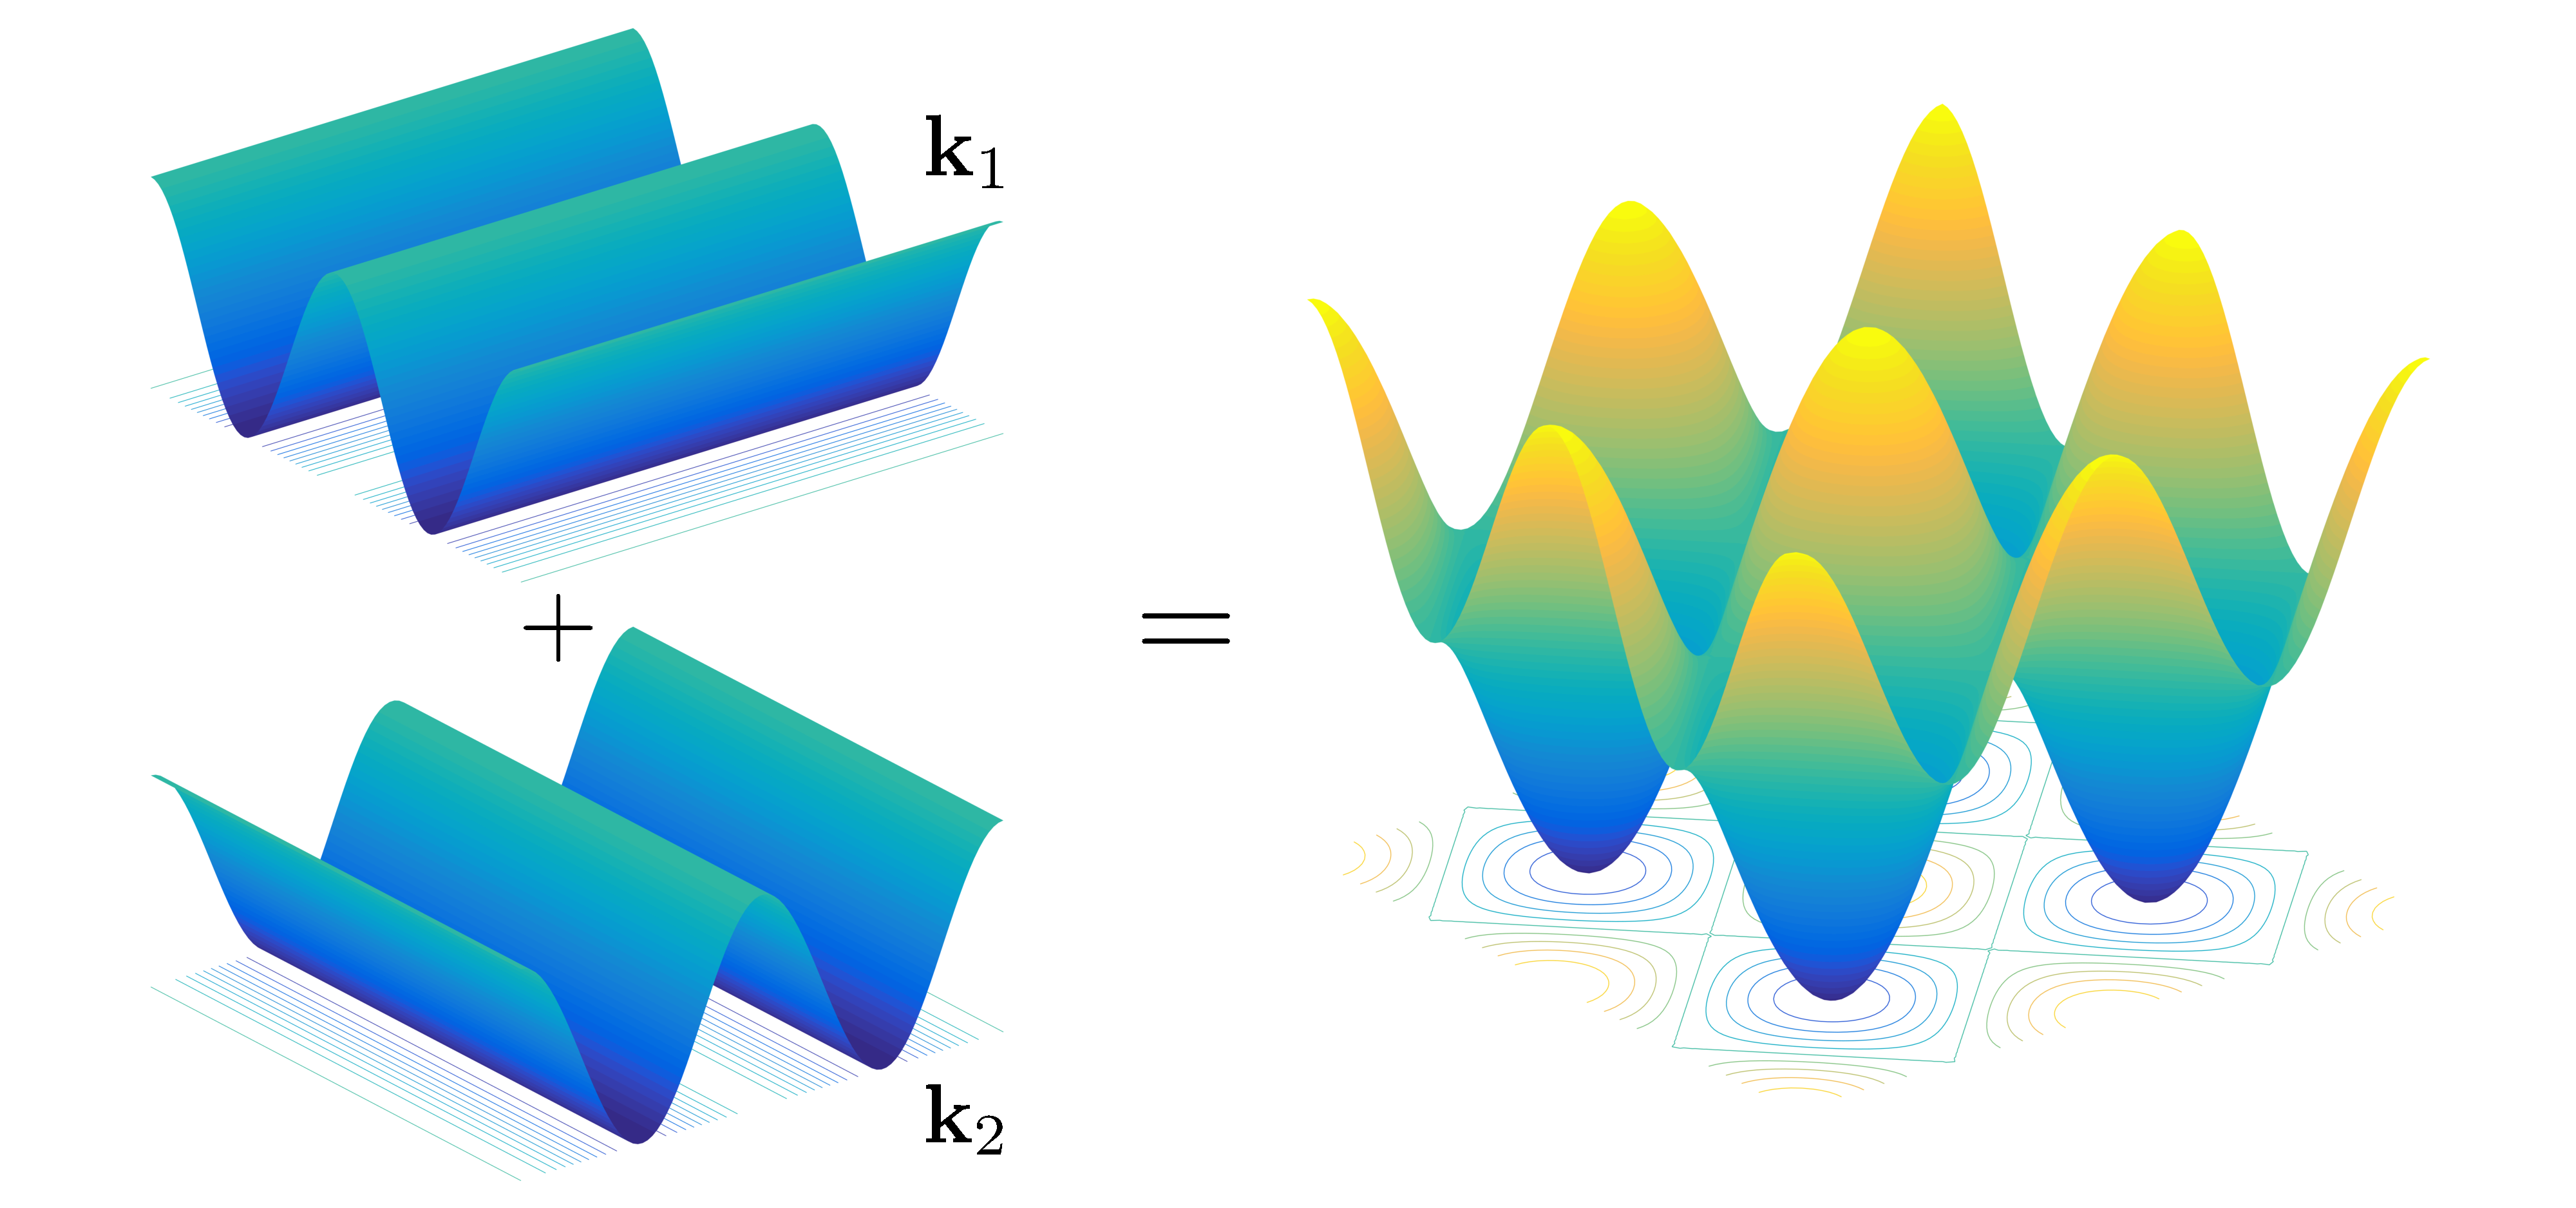
\includegraphics[width=0.55\textwidth]{./Images/ch4_vtx/VOPT/squarelatt}
    \caption{Square lattice generation using two orthogonal propagating laser fields, as defined by Eq.~\ref{eqn:sqlatt}.}\label{fig:cos2xy}
\end{figure}
By choice of $f(t)$, the time of application of the optical lattice to the condensate can be controlled. Given some time for evolution, the wavefunction phase will be modified and evolve due to the presence of the new potential. Of particular interest is the use of an instantaneously switched optical potential. For an optical lattice that is switched on and permanently remains on, such as a quench of the form $f(t) = \Theta(t)$ where $\Theta$ is the Heaviside step function, the condensate will see this and attempt to adjust to the new Hamiltonian. However, for a pulsed optical lattice, such as a $\delta$-function in time, the condensate does not immediately respond, with the resulting \textit{kick} modifying the phase profile of the wavefunction. Experimentally, one can imagine this effect coming from the use of an optical shutter, and thus we can assume this is a realisable perturbation, with the potential intensity controlled by beam power.

\iffalse
For the purpose of my system, I intend to create a two-dimensional optical lattice, wherein the structure of the lattice matches that of the triangular Abrikosov vortex pattern. The triangular lattice has 6-fold rotational symmetry, and can be formed with wavevectors

\begin{subequations}
    \begin{align}
        \mathbf{k}_1 &= k_0\left\{\frac{\sqrt(3)}{2},\frac{1}{2}\right\} \\
        \mathbf{k}_2 &= k_0\{0,1\} \\
        \mathbf{k}_3 &= k_0\left\{\frac{\sqrt(3)}{2},-\frac{1}{2}\right\} \\
    \end{align}
\end{subequations}
where $k_0 = 4\pi/(\sqrt(3)a_0)$, and $a_0$ is the lattice spacing.
\fi


%%%%%%%%%%%%%%%%%%%%%%%%%%%%%%%%%%%%%%%%%%%%%%%%%%%%%%%%%%%% b
\subsection{Direct phase manipulation}\label{sec:phase}
%%%%%%%%%%%%%%%%%%%%%%%%%%%%%%%%%%%%%%%%%%%%%%%%%%%%%%%%%%%%

While groundstate condensates will have a flat phase across the system, there are some interesting examples where a spatially dependent phase exists: dark solitons and vortices. I have previously discussed the $2\pi$ phase profile of a vortex. Dark solitons are another type of topological excitation that feature a $\pi$ phase jump profile. These excitations are unstable in dimensions higher than one, and will decay via a snake instability to paired vortices and antivortices [citation], as shown in Fig.~\ref{fig:solitons}.

\begin{figure}\centering
    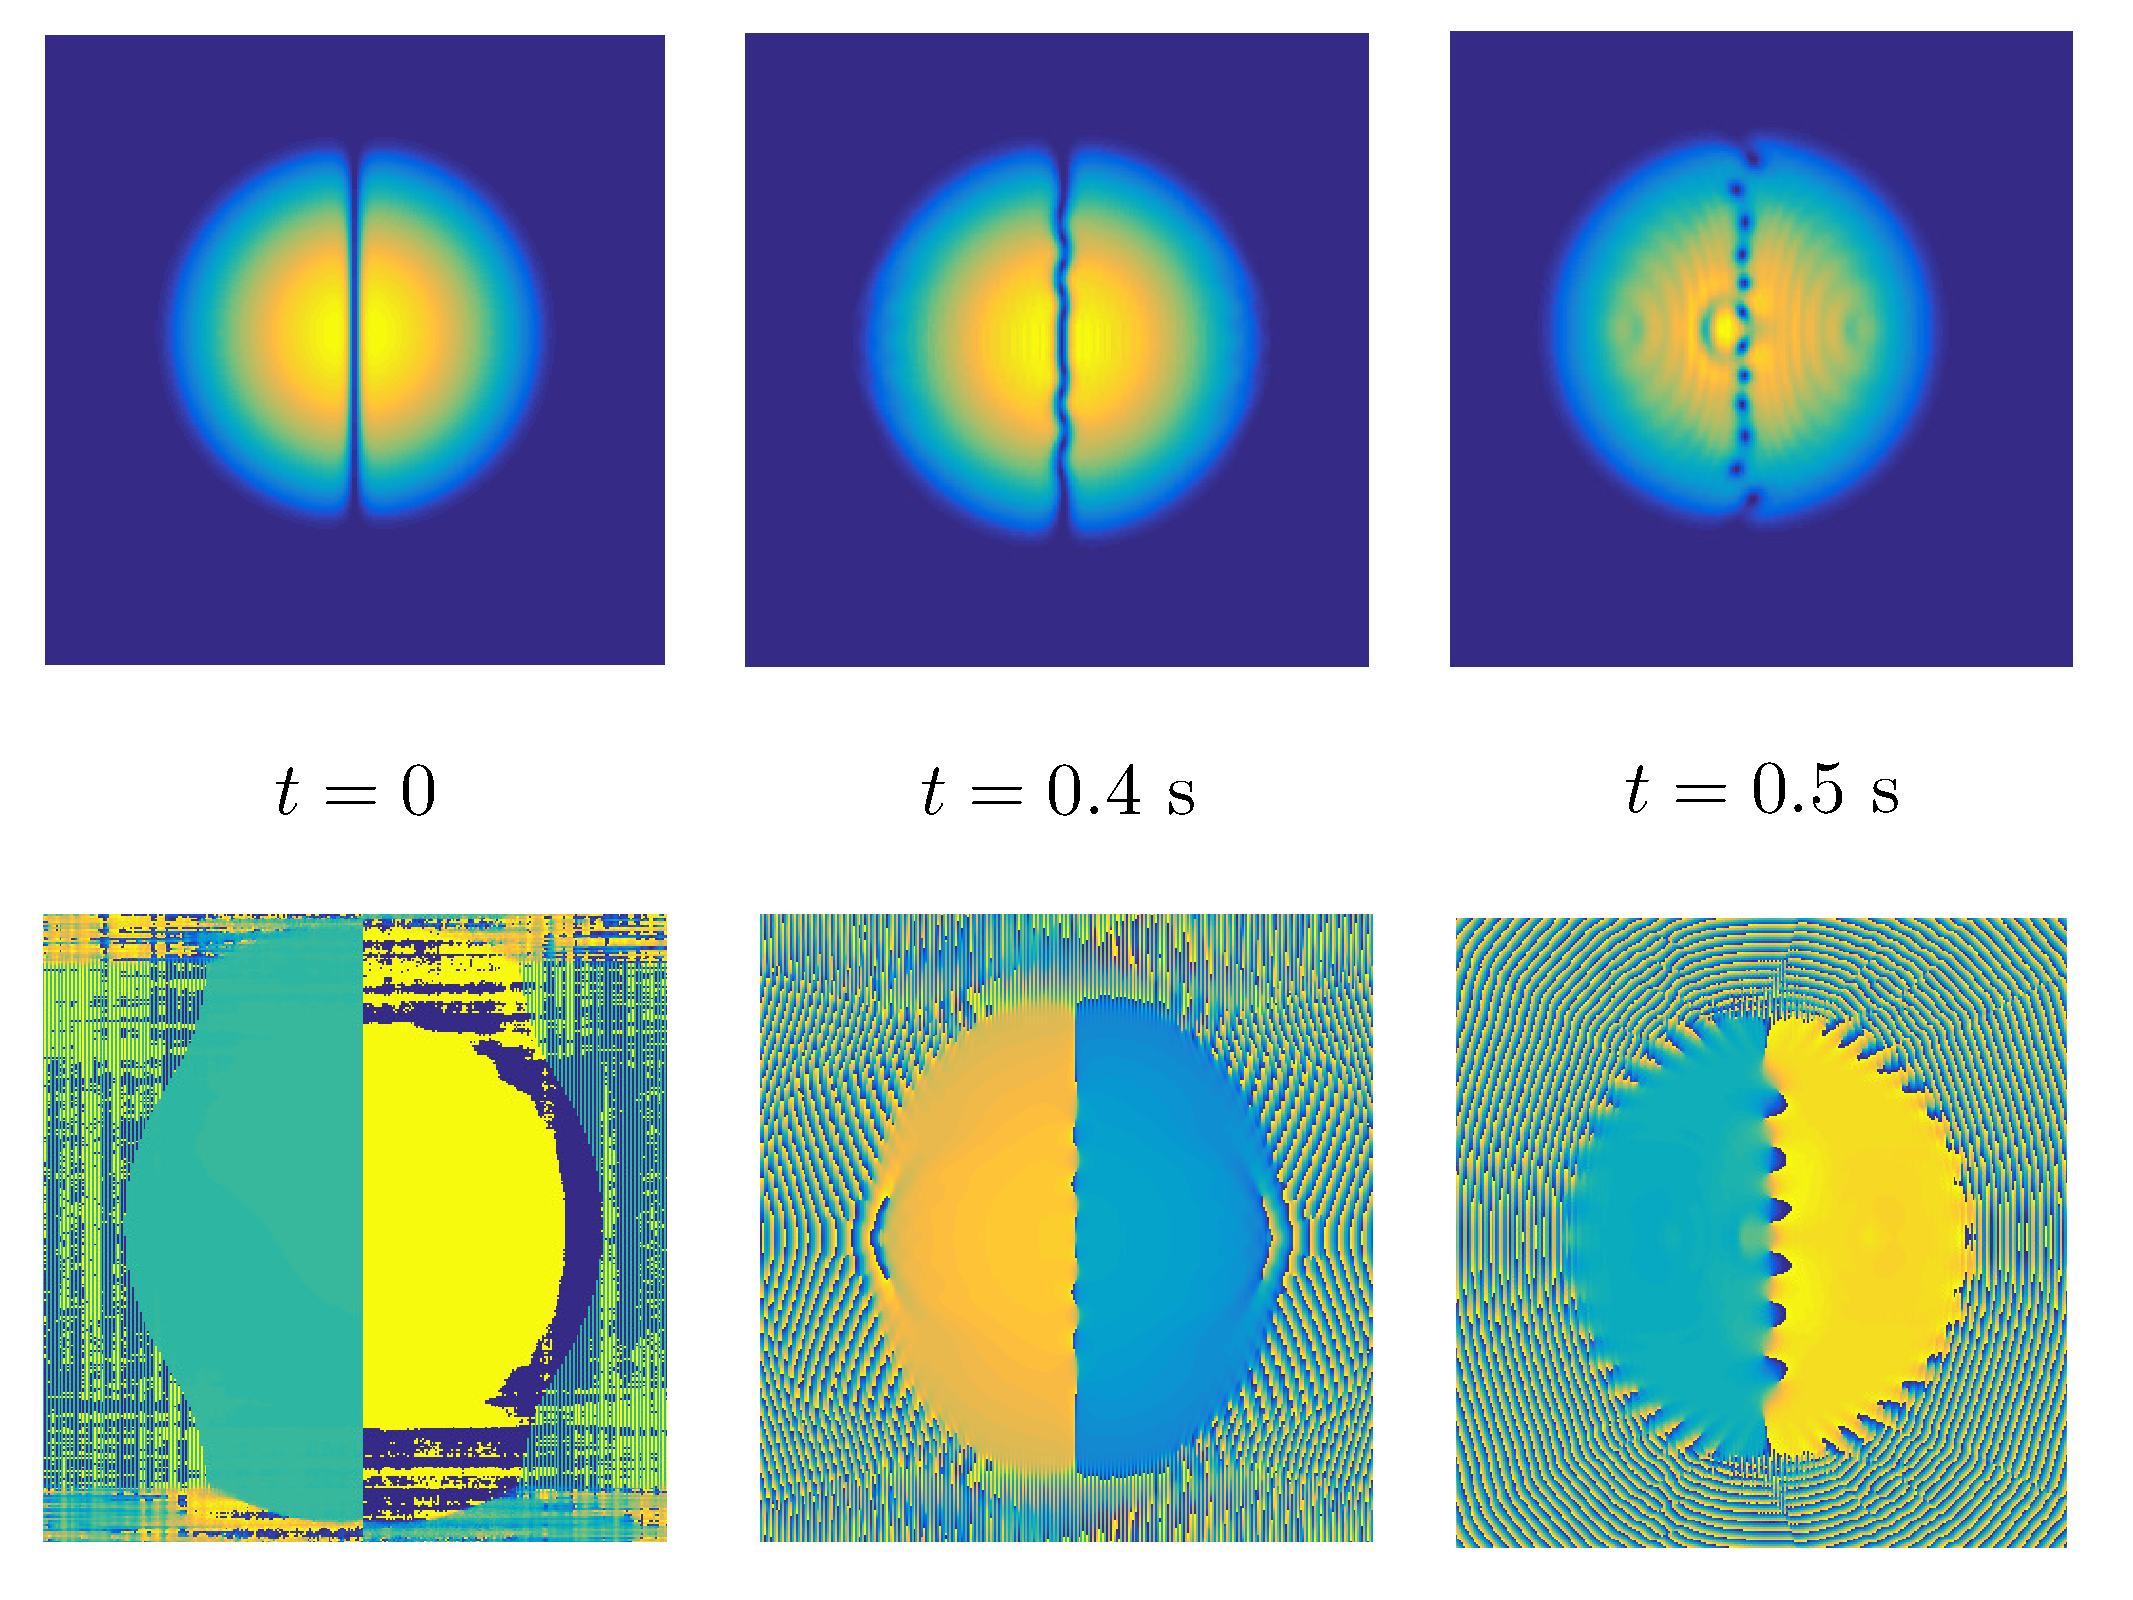
\includegraphics[width=0.75\textwidth]{Images/ch4_vtx/solitons.pdf}
    \caption{A dark soliton in two-dimensions decaying via the snake instability to pairs of vortices and antivortices. The density (top) and phase (bottom) are given for times $t=0,0.4,0.5$ s.}\label{fig:solitons}
\end{figure}

Where previously I have considered the evolution of the wavefunction in the presence of a kicked smoothly varying optical potential, one can also consider the case of a directly imprinted phase. Phase imprinting is a technique that applies a spatially inhomogeneous potential across a condensate in such a way that the phase is modified to a desired form. As a consequence the density distribution will adjust itself in time and dark solitons \cite{BEC:Denschlag_science_2000}, as well as vortices \cite{Vtx:Dobrek_pra_1999} have been created this way. For the latter the signature is given by a phase singularity, around which the phase winds through $\pm 2\pi$, depending upon the direction of rotation. As discussed in Sec.~\ref{sec:}, this is the phase profile given for a quantum vortex, and by application of this pattern one can create such a topological defect in the wavefunction.

Following \cite{BK:Pitaevskii_Stringari_2003} and taking the Madelung transform of the wavefunction given by Eq. \eqref{eqn:madelung}, the phase of the condensate may be specified as
\begin{equation}
\theta = \theta_0 + \theta_i,
\end{equation}
where $\theta_0$ is the unperturbed condensate phase, and $\theta_i$ is the phase pattern to be imprinted. Usually $\theta_0$ is constant allowing the simple addition of features such as vortices and solitons to a condensate wavefunction. Upon solving for the initial condensate groundstate with deterministic phase, an additional phase pattern can be imprinted at any time by multiplying the wavefunction by $e^{\text{i}\theta_i}$. More generally, without careful choice of the phase terms their addition can lead to a mess, so care must be taken to choose a well defined initial and imprinting phase pattern.

Though in Sec.~\ref{ss:pert_opt_latt} I added an optical potential to the Hamiltonian for a short time during the evolution, here I directly engineer the wavefunction phase. The advantage of the phase imprinting model is that for topological defects, one can essentially imprint the required winding instantaneously. The density also need only adjust itself local to the phase singularity, with the remaining condensate seeing an almost constant shift in phase.

The creation of vortices through application of localised $\pm 2\pi$ phase winding defects in the condensate allows for direct control of the angular momentum and vorticity of the BEC. Given the rapid change of the phase, and hence the kinetic energy of the condensate, the appearance of phonons are expected following the imprint. While it has been discussed in the literature for creation of vortices, the phase imprinting method can also be used to annihilate a vortex from the condensate by applying a phase profile of opposite winding, removing the singularity. This will leave the condensate with a density depletion at the prior location of the phase singularity. Without the singularity this depletion will fill in and excite phonon modes in the condensate during time evolution. This method will form the basis for which the further discussions and analysis are performed on the vortex carrying condensate.

Experimental realisation of arbitrary phase patterns are accessible through the use of spatial light modulators (SLM). These devices behave as digital displays, through which any visual pattern can be expressed, allowing the masking of a laser field to the required form. I will assume for all future discussions that the potentials are experimentally realisable, and focus on the resulting effect on the condensate. For the creation of a single vortex the $2\pi$ phase winding pattern can be created spatially using
\begin{equation}
    \theta_i(\mathbf{x},\mathbf{y},x_0,y_0) = \atantwo(\mathbf{y}-y_0,\mathbf{x}-x_0),
\end{equation}
where the singularity is located at the position $\left(x_0,y_0\right)$. The resulting phase is shown by Fig.~\ref{fig:atan2phase}.
\begin{figure}\centering
    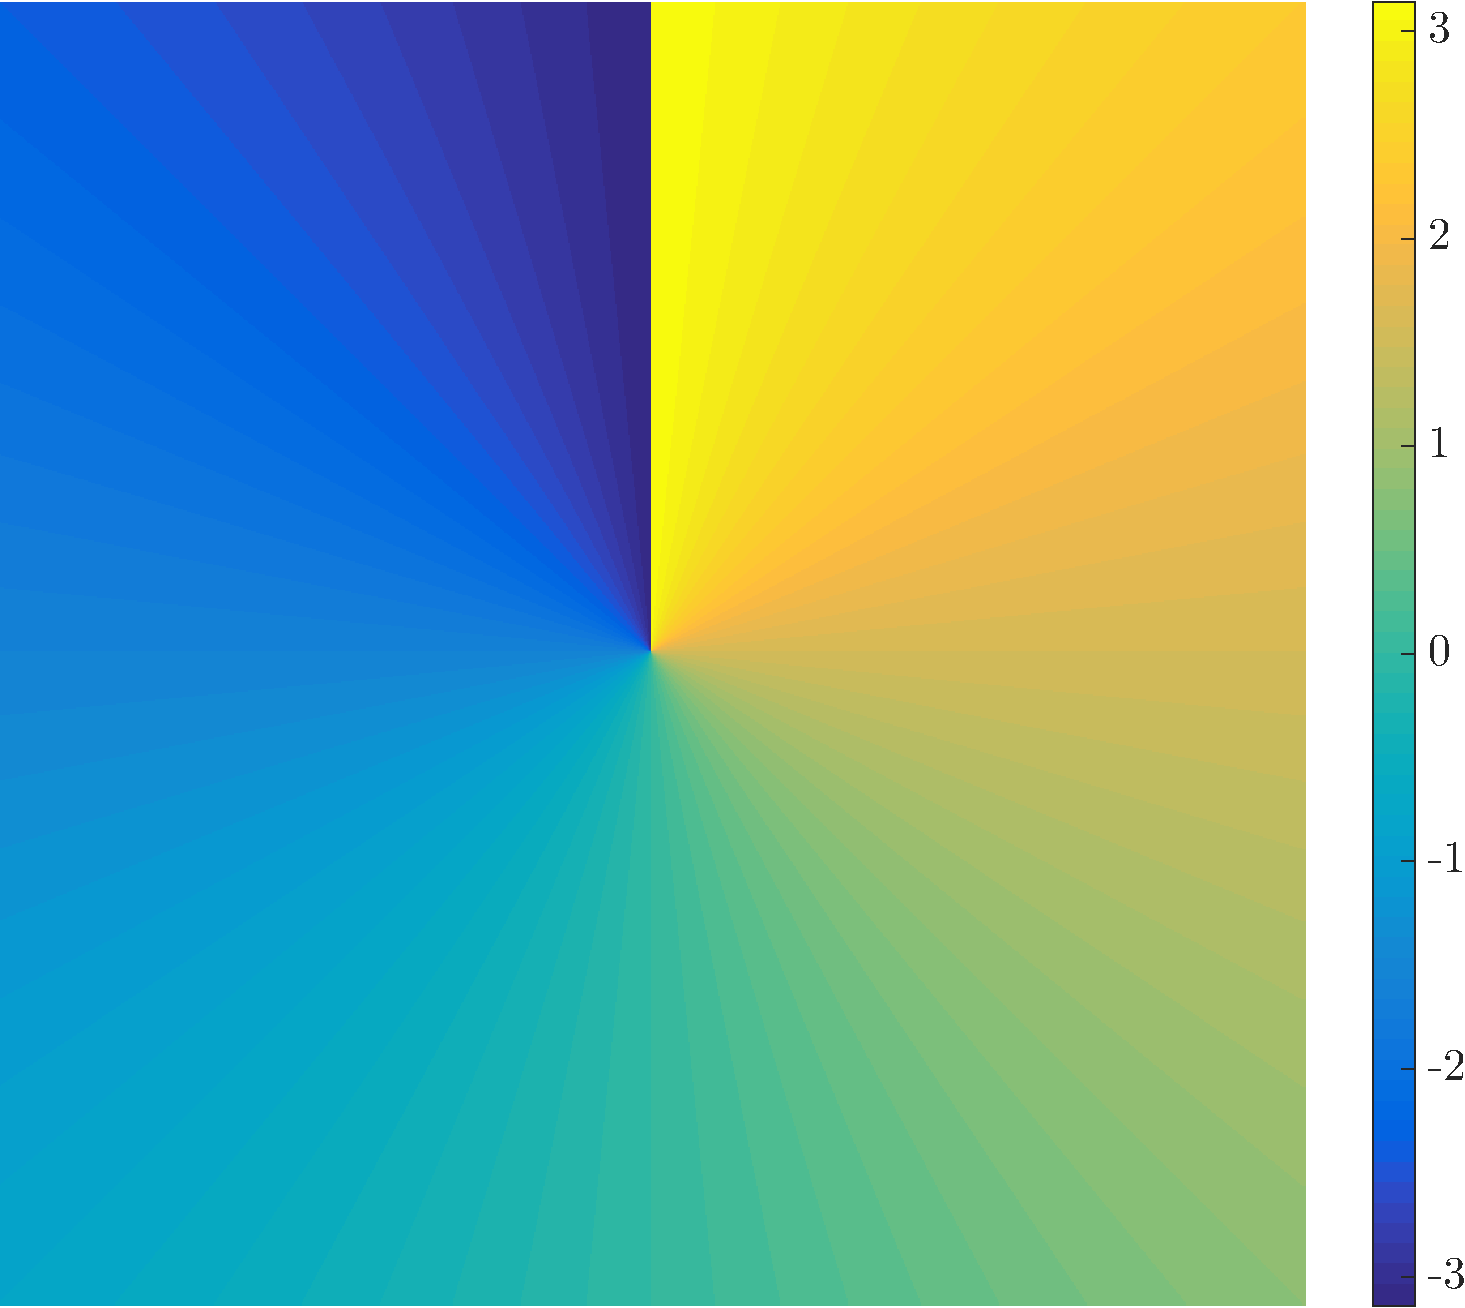
\includegraphics[width=0.45\textwidth]{Images/ch4_vtx/2pi.pdf}
    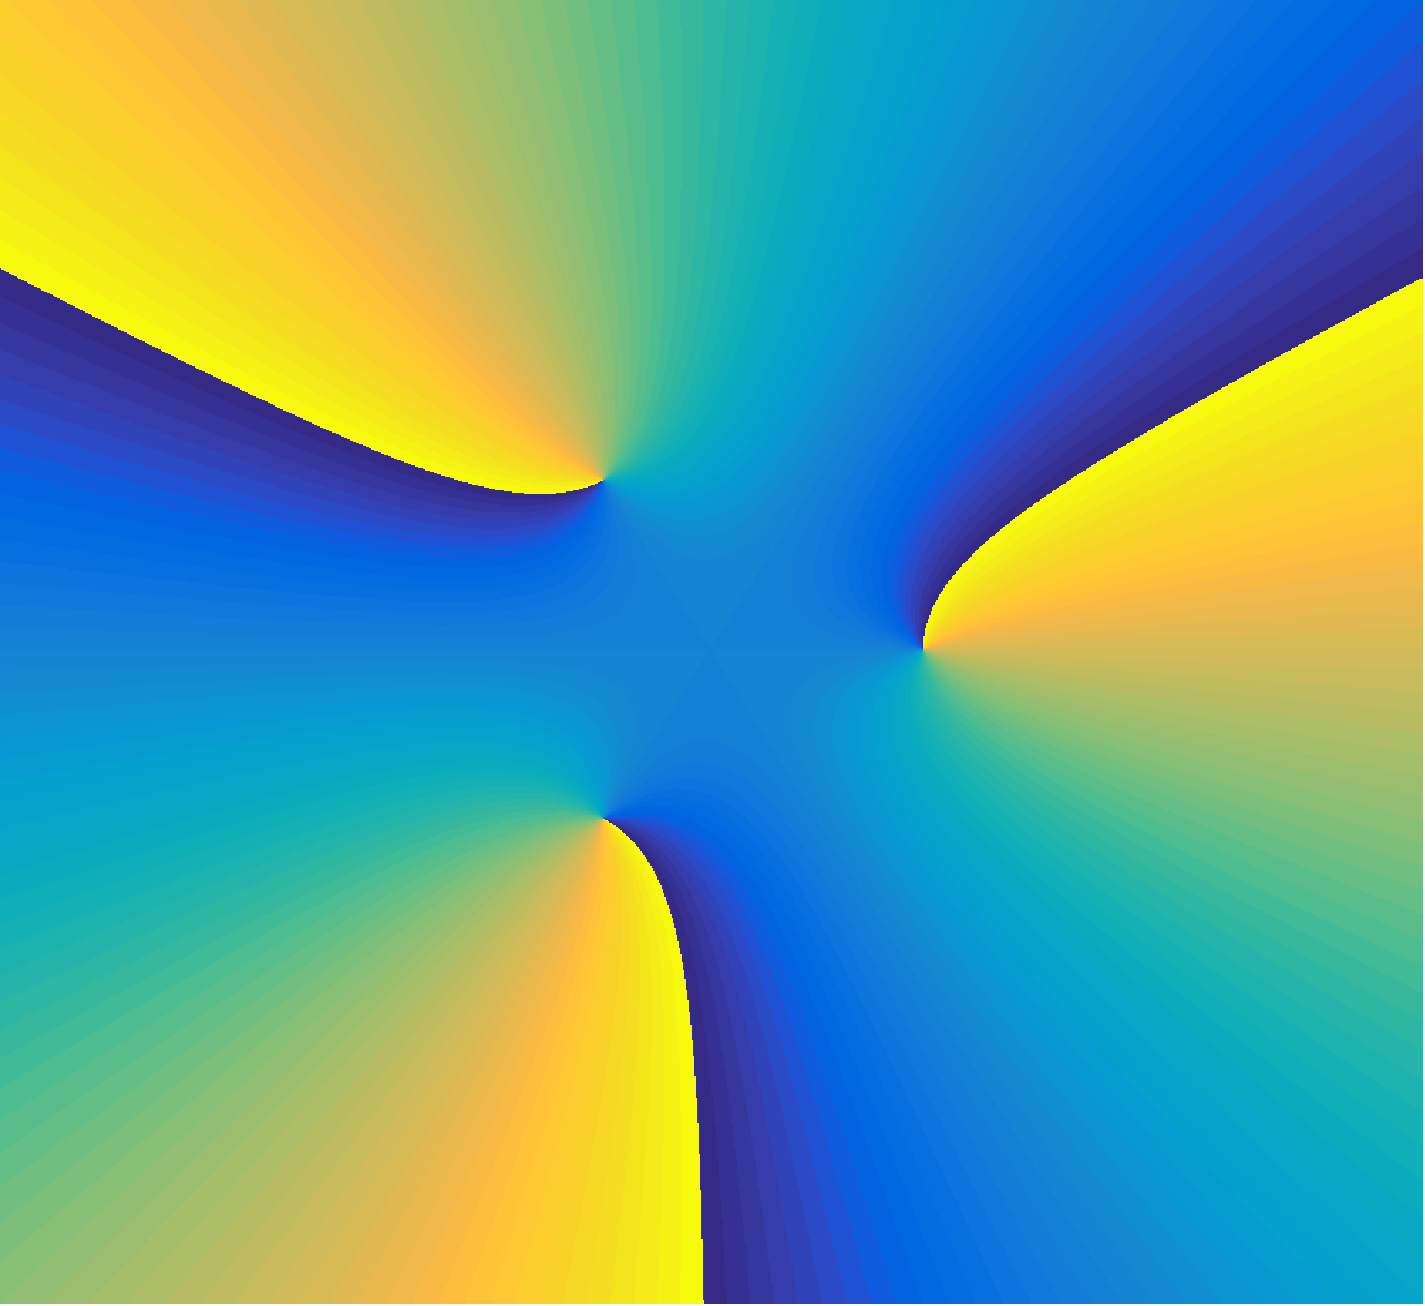
\includegraphics[width=0.435\textwidth]{Images/ch4_vtx/3_2pi.pdf}
    \caption{The $2\pi$ phase winding is shown for a single (left) and three separated (right) phase singularities. The application of separate phase singularities can be treated as summing each individual phase profile, $\displaystyle\sum\limits_i \theta_i \mod 2\pi$.}\label{fig:atan2phase}
\end{figure}
Writing the wavefunction in the standard Madelung transform form, and including the additional phase singularity term $\theta_i$, I imprint this singularity to the condensate wavefunction as
\begin{equation}
    \Psi(\mathbf{r},t) = |\Psi(\mathbf{r},t)|e^{\text{i}(\theta_0(\mathbf{r},t) + \theta_i(\mathbf{r}))}.
\end{equation}
An example of this is given in Fig.~\ref{fig:0to1vtx}, where the condensate density and phase is shown, following imaginary time evolution, before and after a phase imprint.

\begin{figure}\centering
    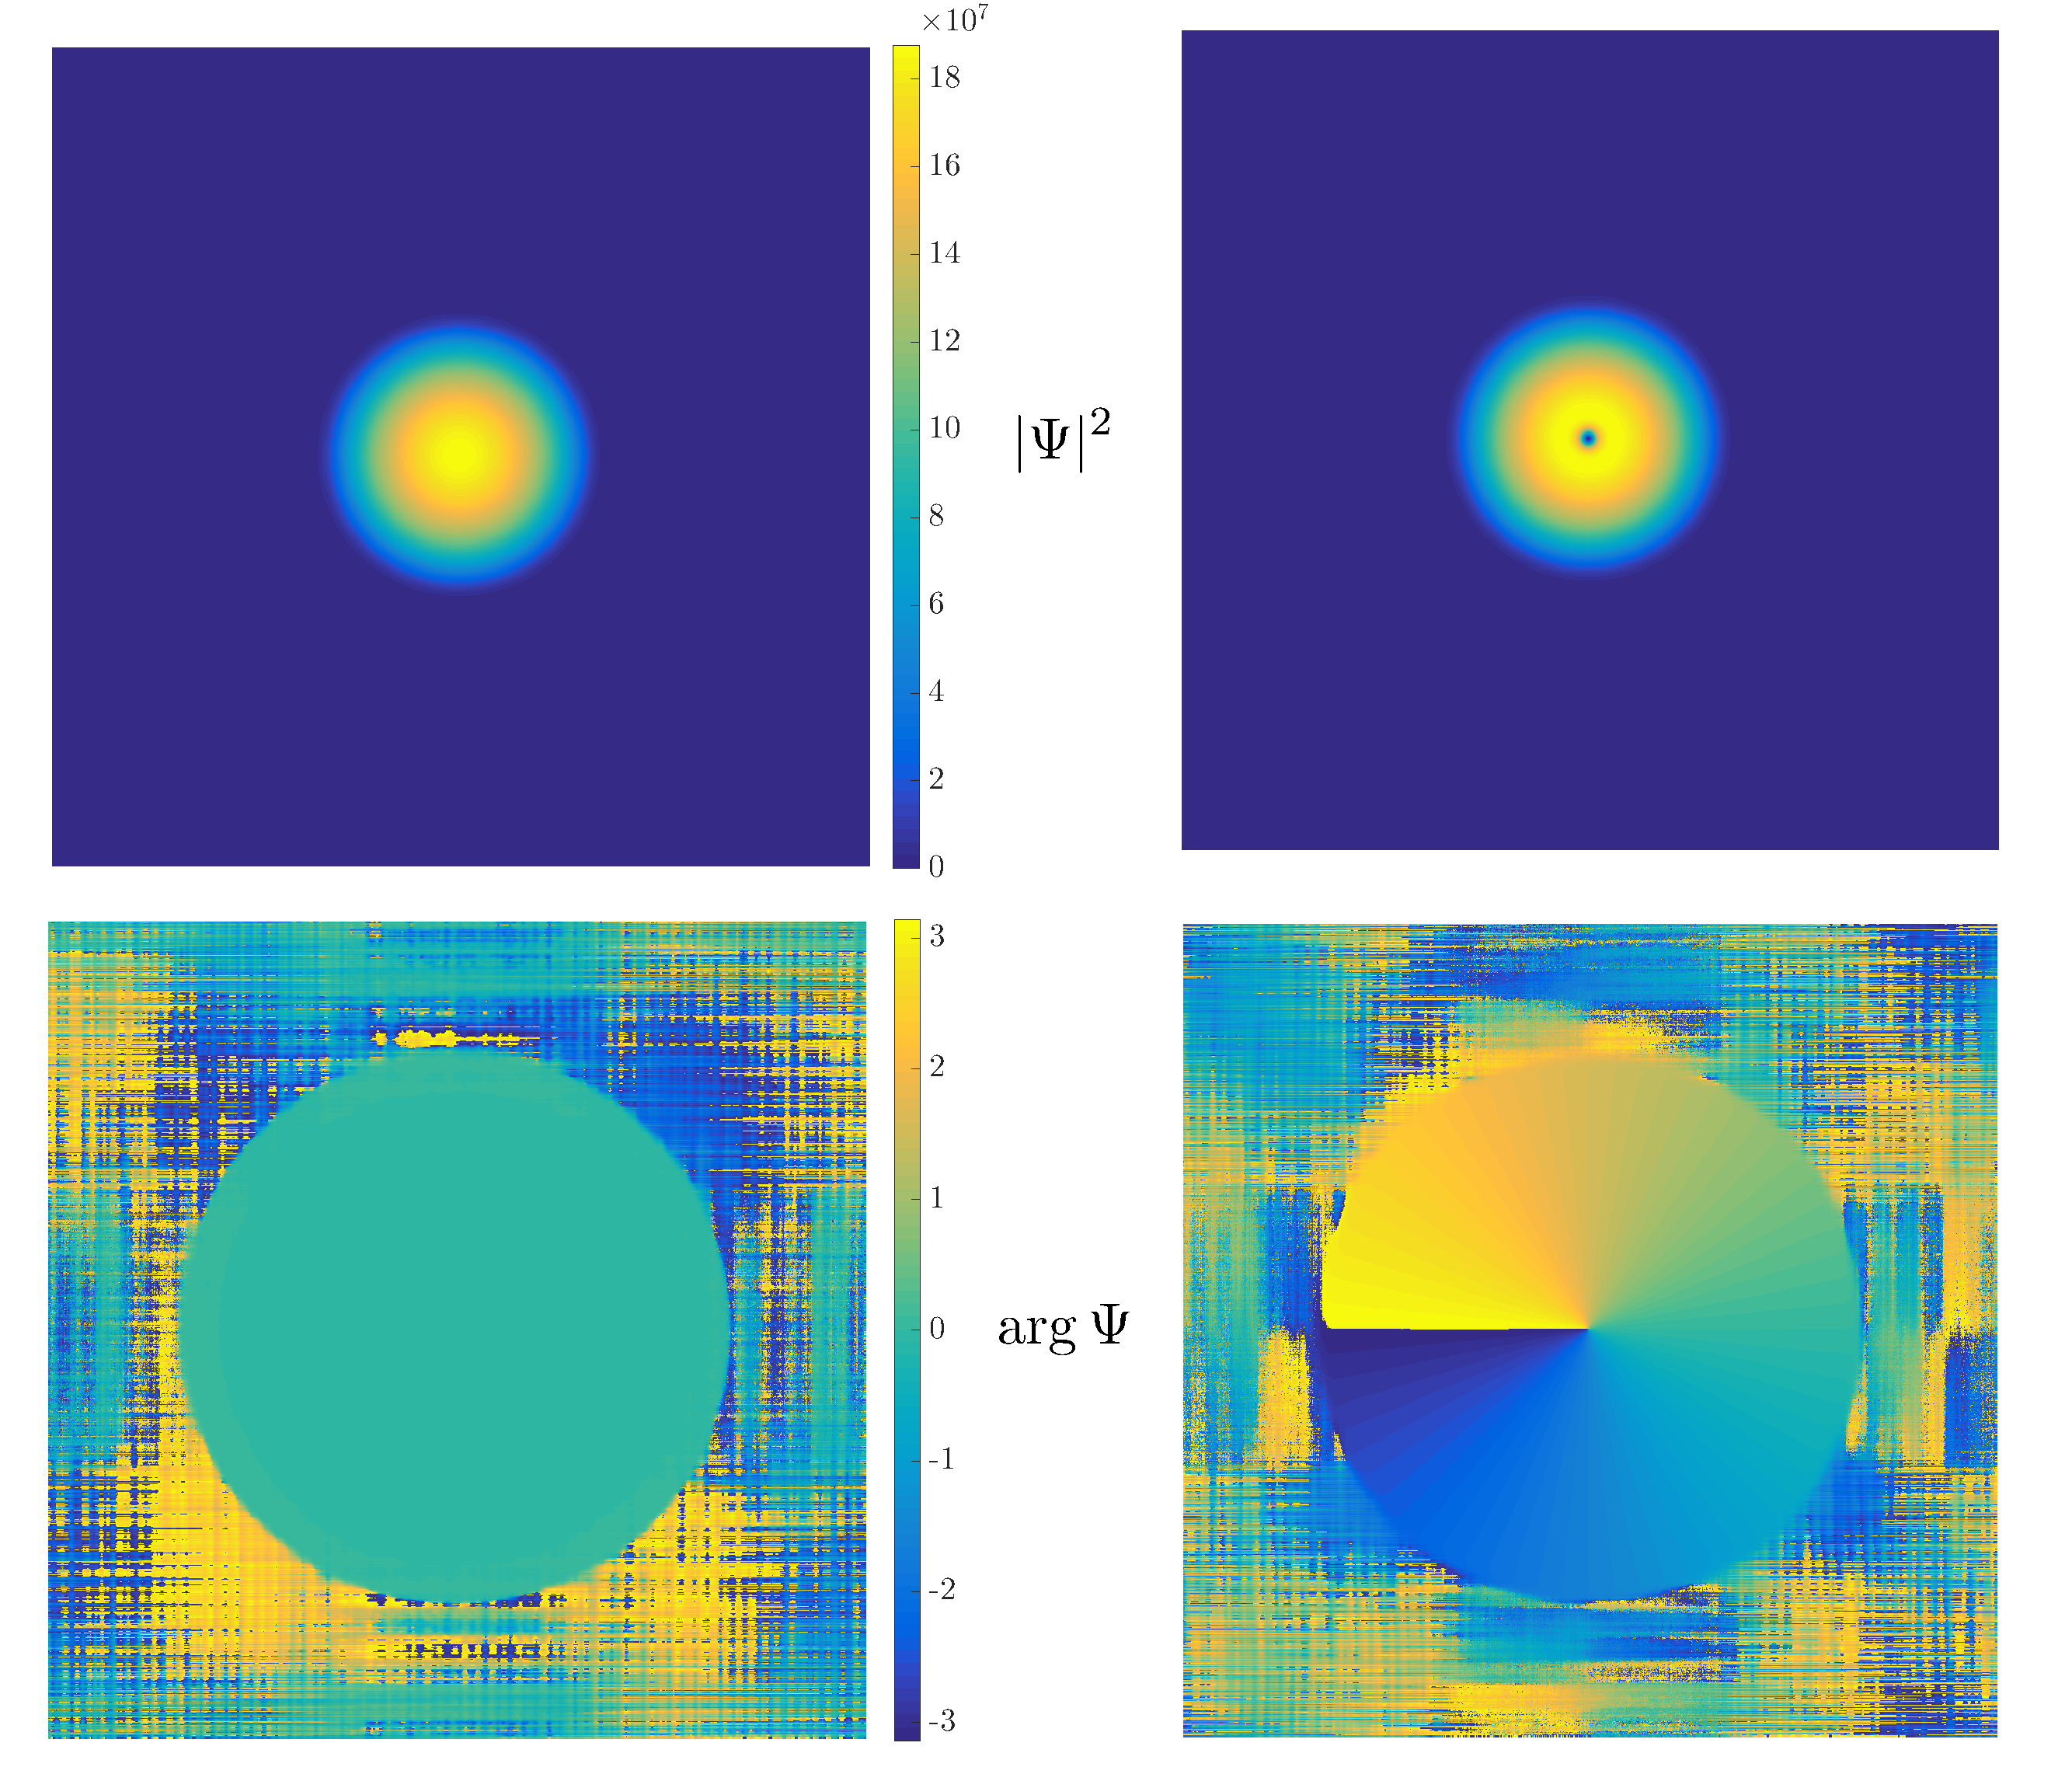
\includegraphics[width=0.75\textwidth]{Images/ch4_vtx/1vtxbec.pdf}
    \caption{The condensate density and phase are shown in the absence and presence of a vortex. The density dip location corresponds exactly with the phase singularity, around which it winds from $-\pi$ to $\pi$}.\label{fig:0to1vtx}
\end{figure}
While here I have shown the creation of a groundstate solution with the phase imprint and imaginary time evolution, this process may also be carried out during real-time evolution, though with the addition of phonons in the density resulting from the imprint. For a closed system the vortex imprint will raise the energy of the system, and likely not be a groundstate.

As imprinting is directly controlling the condensate phase, given the dependence of superfluid velocity on the phase gradient, any change can also be considered a direct manipulation of the kinetic energy. By applying spatially inhomogeneous phase profiles the atomic velocity can be adjusted to different values in different regions of the condensate. One such example I will consider is that of the application of a Gaussian phase profile to the condensate, of the form

\begin{equation}
    \theta^{(i)}(\mathbf{r}) = A\exp\left( -\frac{ |\mathbf{r}-\mathbf{r}_0|^2 }{2\sigma^2 } \right) \mod 2\pi
\end{equation}
with $A$ as the phase profile amplitude, $\mathbf{r}_0$ as the centre of the Gaussian curve, and $\sigma$ adjusted to match the condensate width. The modulo $2\pi$ ensures that the phase wraps around for amplitudes exceeding $(0,2\pi)$ range. The Gaussian profile has large gradients in a ring-shaped geometry in two-dimensions, with the effect of an imprint on the condensate being an expansion of the cloud in a non-homogeneous manner, given the new spatially dependent velocity (see Fig.~\ref{fig:gaussian}). Following the variation in phase profiles, and hence velocities, the condensate is expected to develop interference fringes, as the faster moving atoms overtake the slower ones, for sufficiently large amplitudes. This can be seen in \ref{fig:gaussian_wfc}, where a slice through the condensate centre is given for both position and momentum space. Stronger kicks allow for the onset of interference fringes to develop, with the sign of the imprint indicating the direction of the velocity field. Given the symmetry of the fringes, the clarity of rings could potentially be used to determine the quality of the trapping potentials in experimental setups. This method is of limited availability though as an actual interferometer for other setups, given that the arms would be inside the condensate.

\begin{figure}\centering
    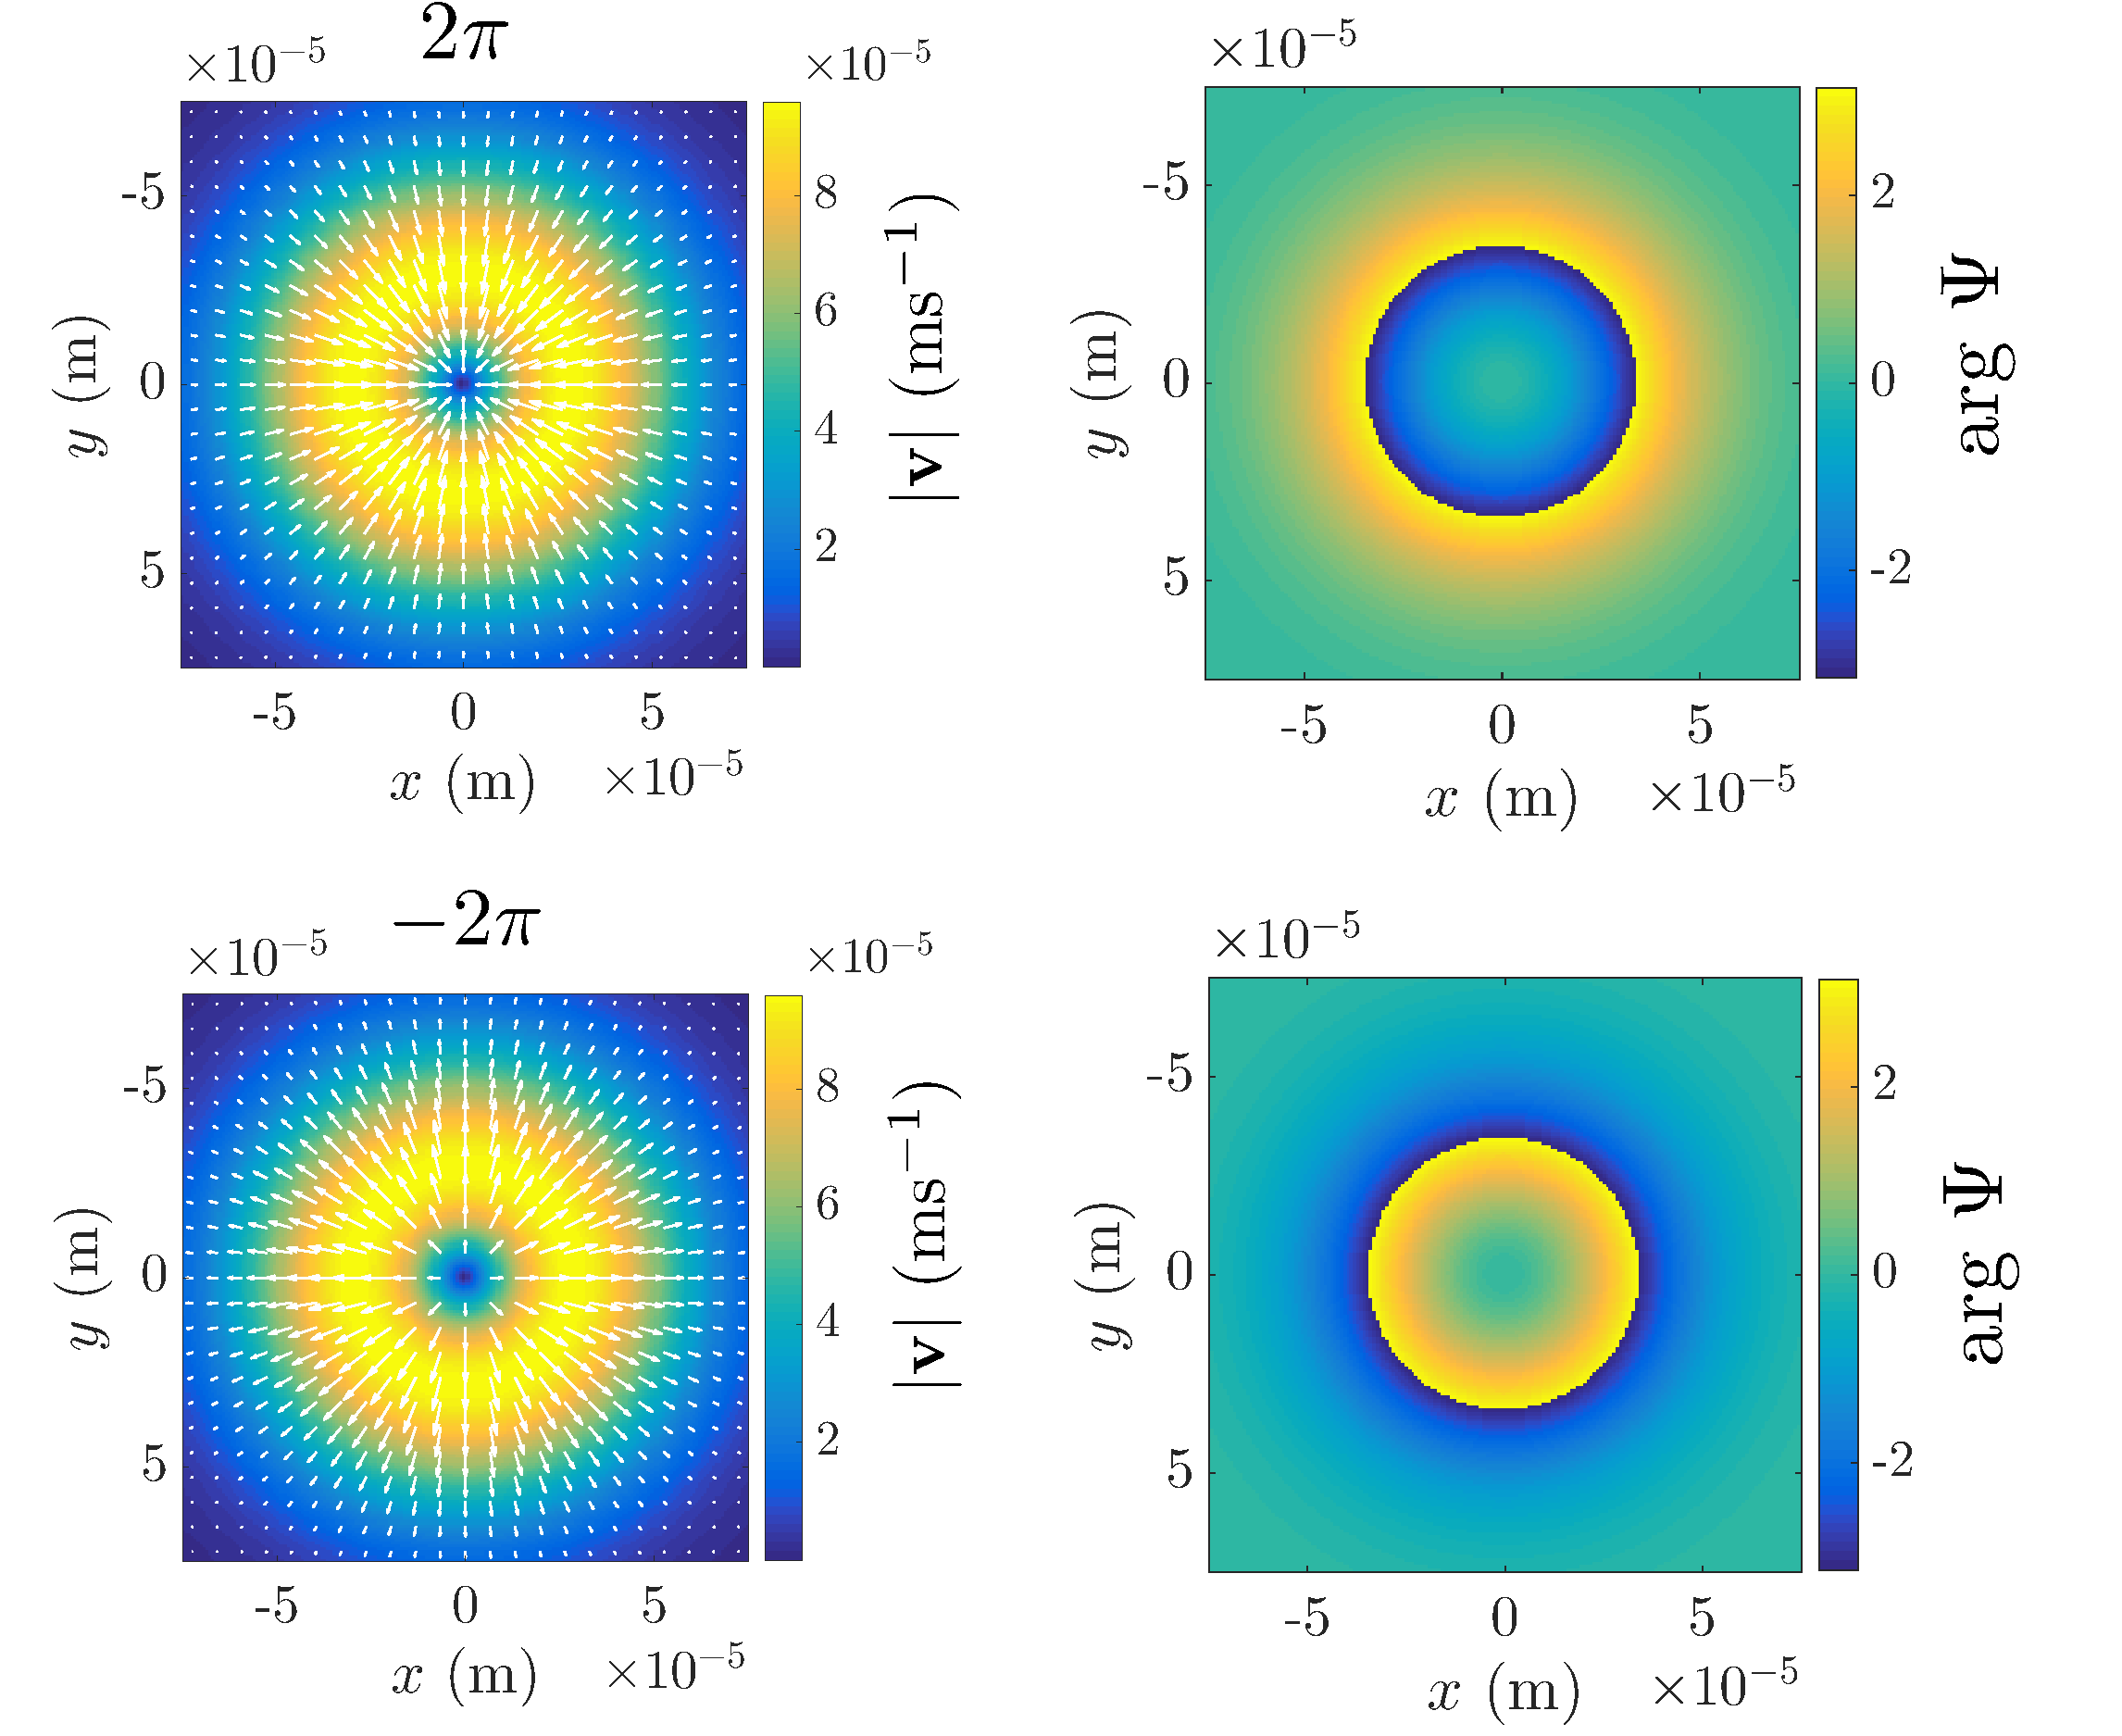
\includegraphics[width=0.95\textwidth]{Images/ch4_vtx/velocity/gaussian_imprint}
    \caption{The velocity fields and magnitude (left) as well as the phase (right) for a condensate following a Gaussian. The sign of the imprint changes the direction of the respective kinetic components, and hence direction of the flow}.\label{fig:gaussian}
\end{figure}


\begin{figure}\centering
    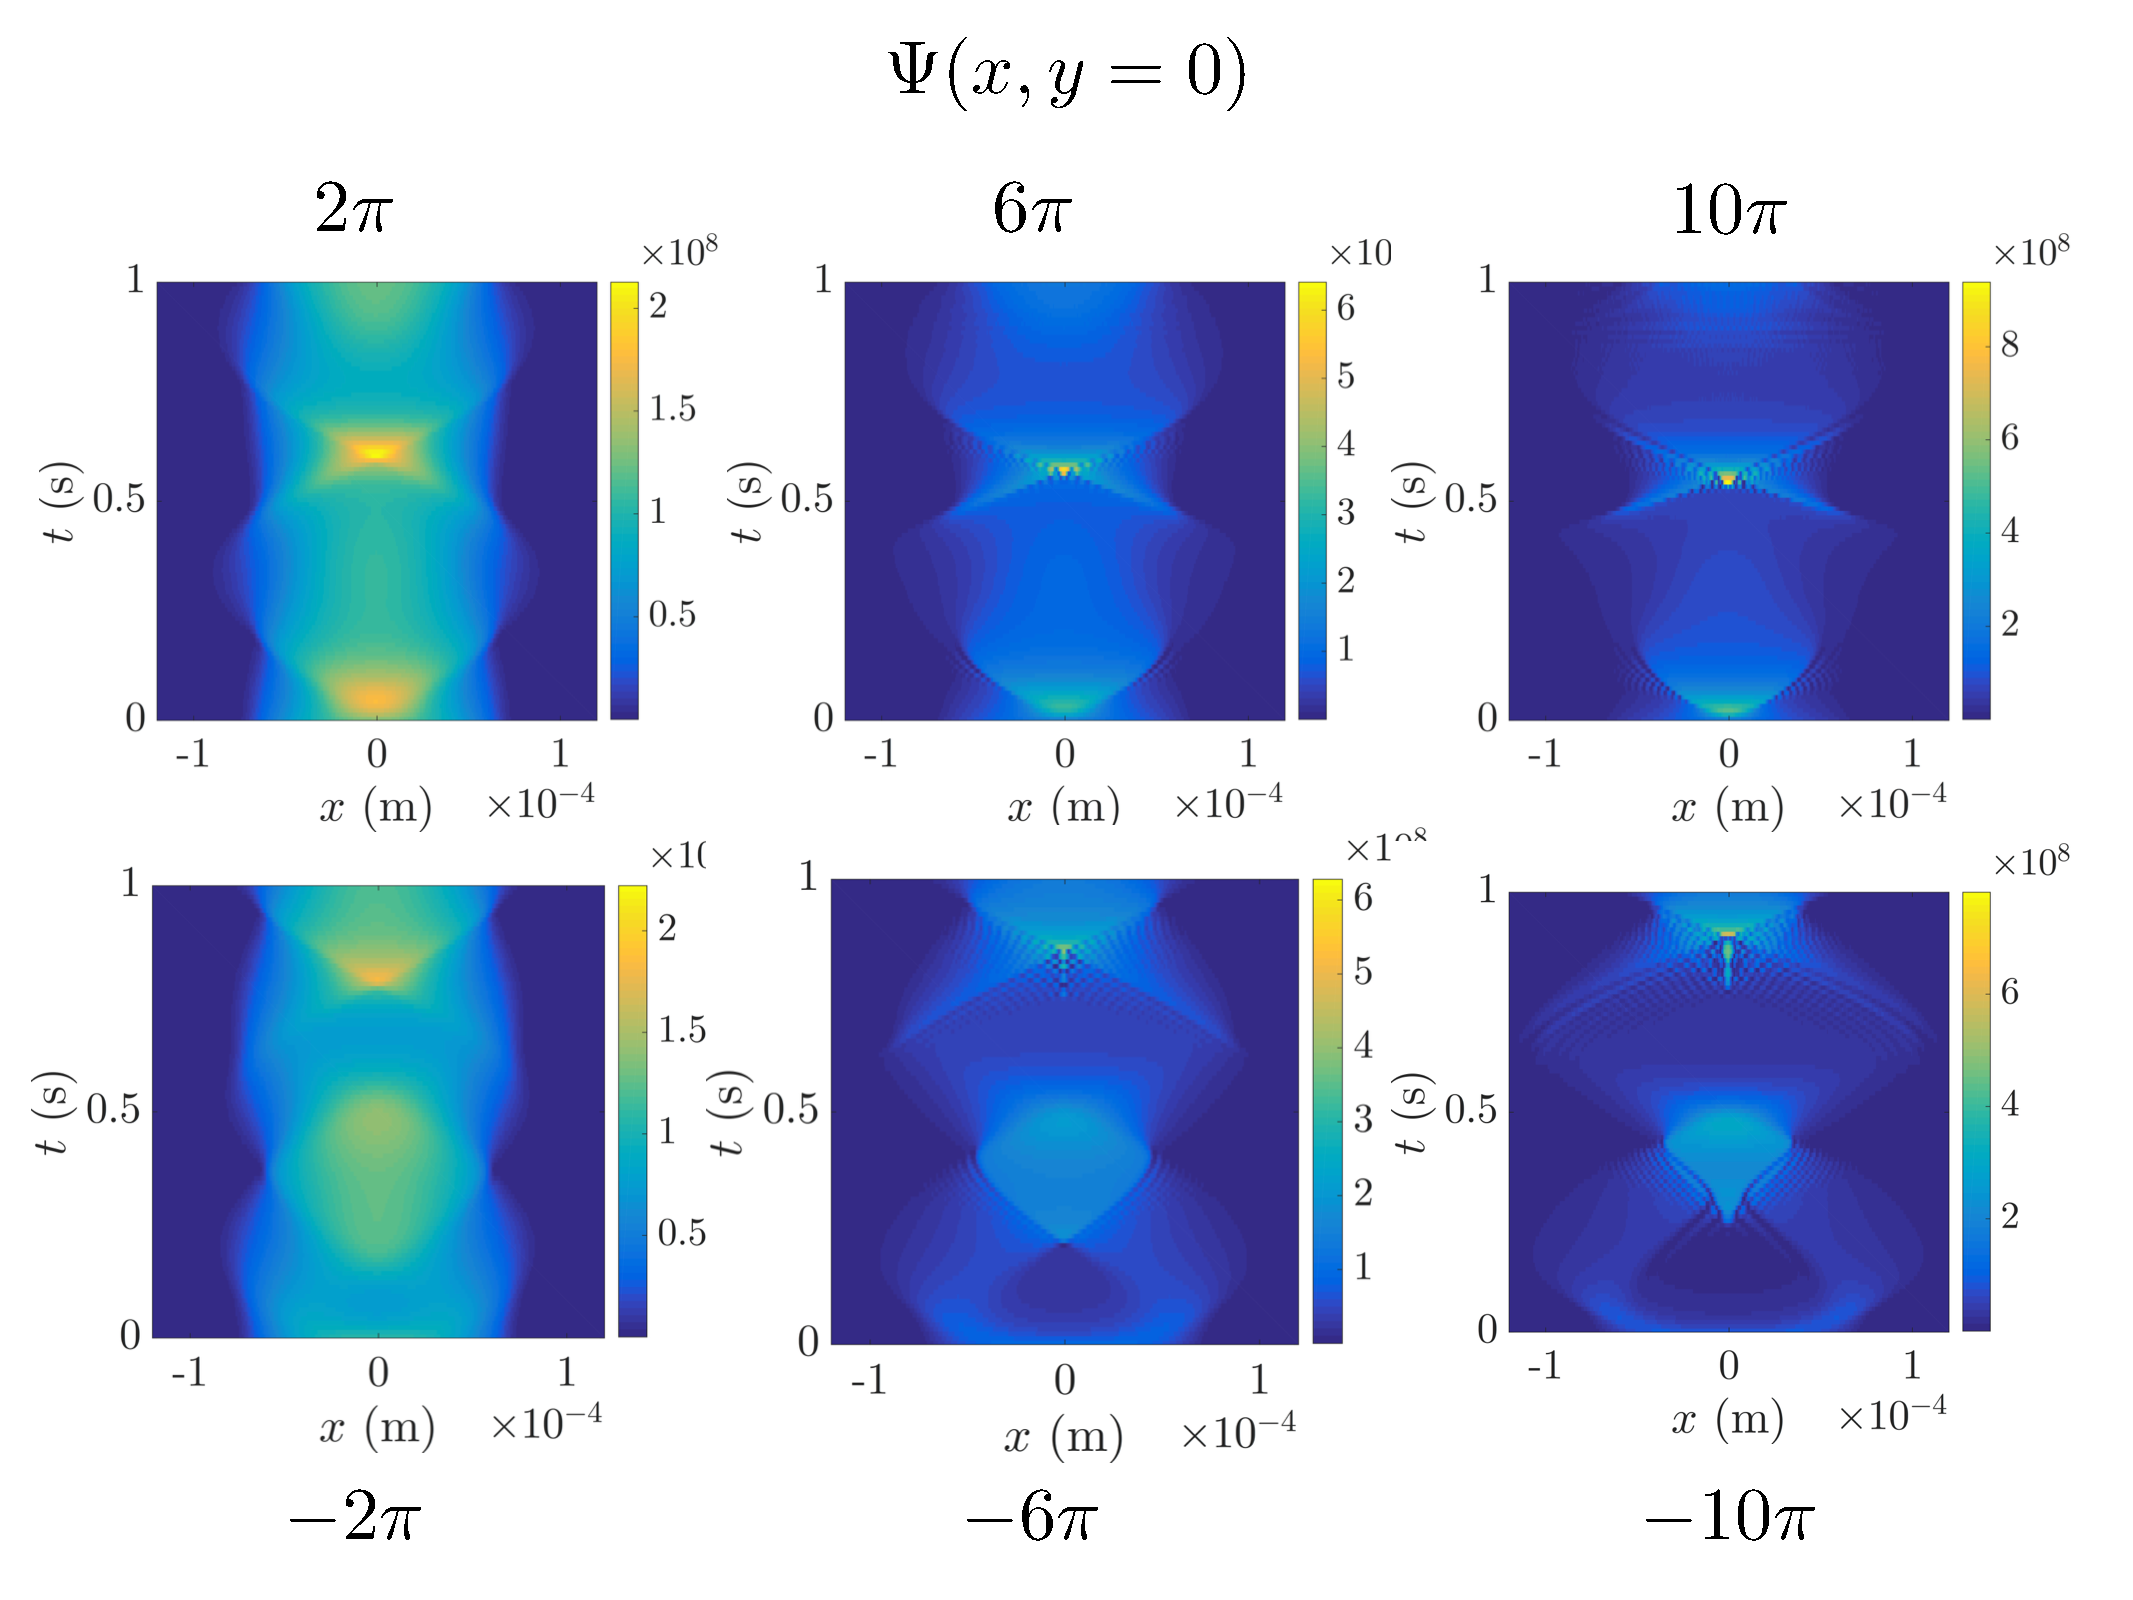
\includegraphics[width=0.95\textwidth]{Images/ch4_vtx/velocity/gaussian_imprint_wfcr}
    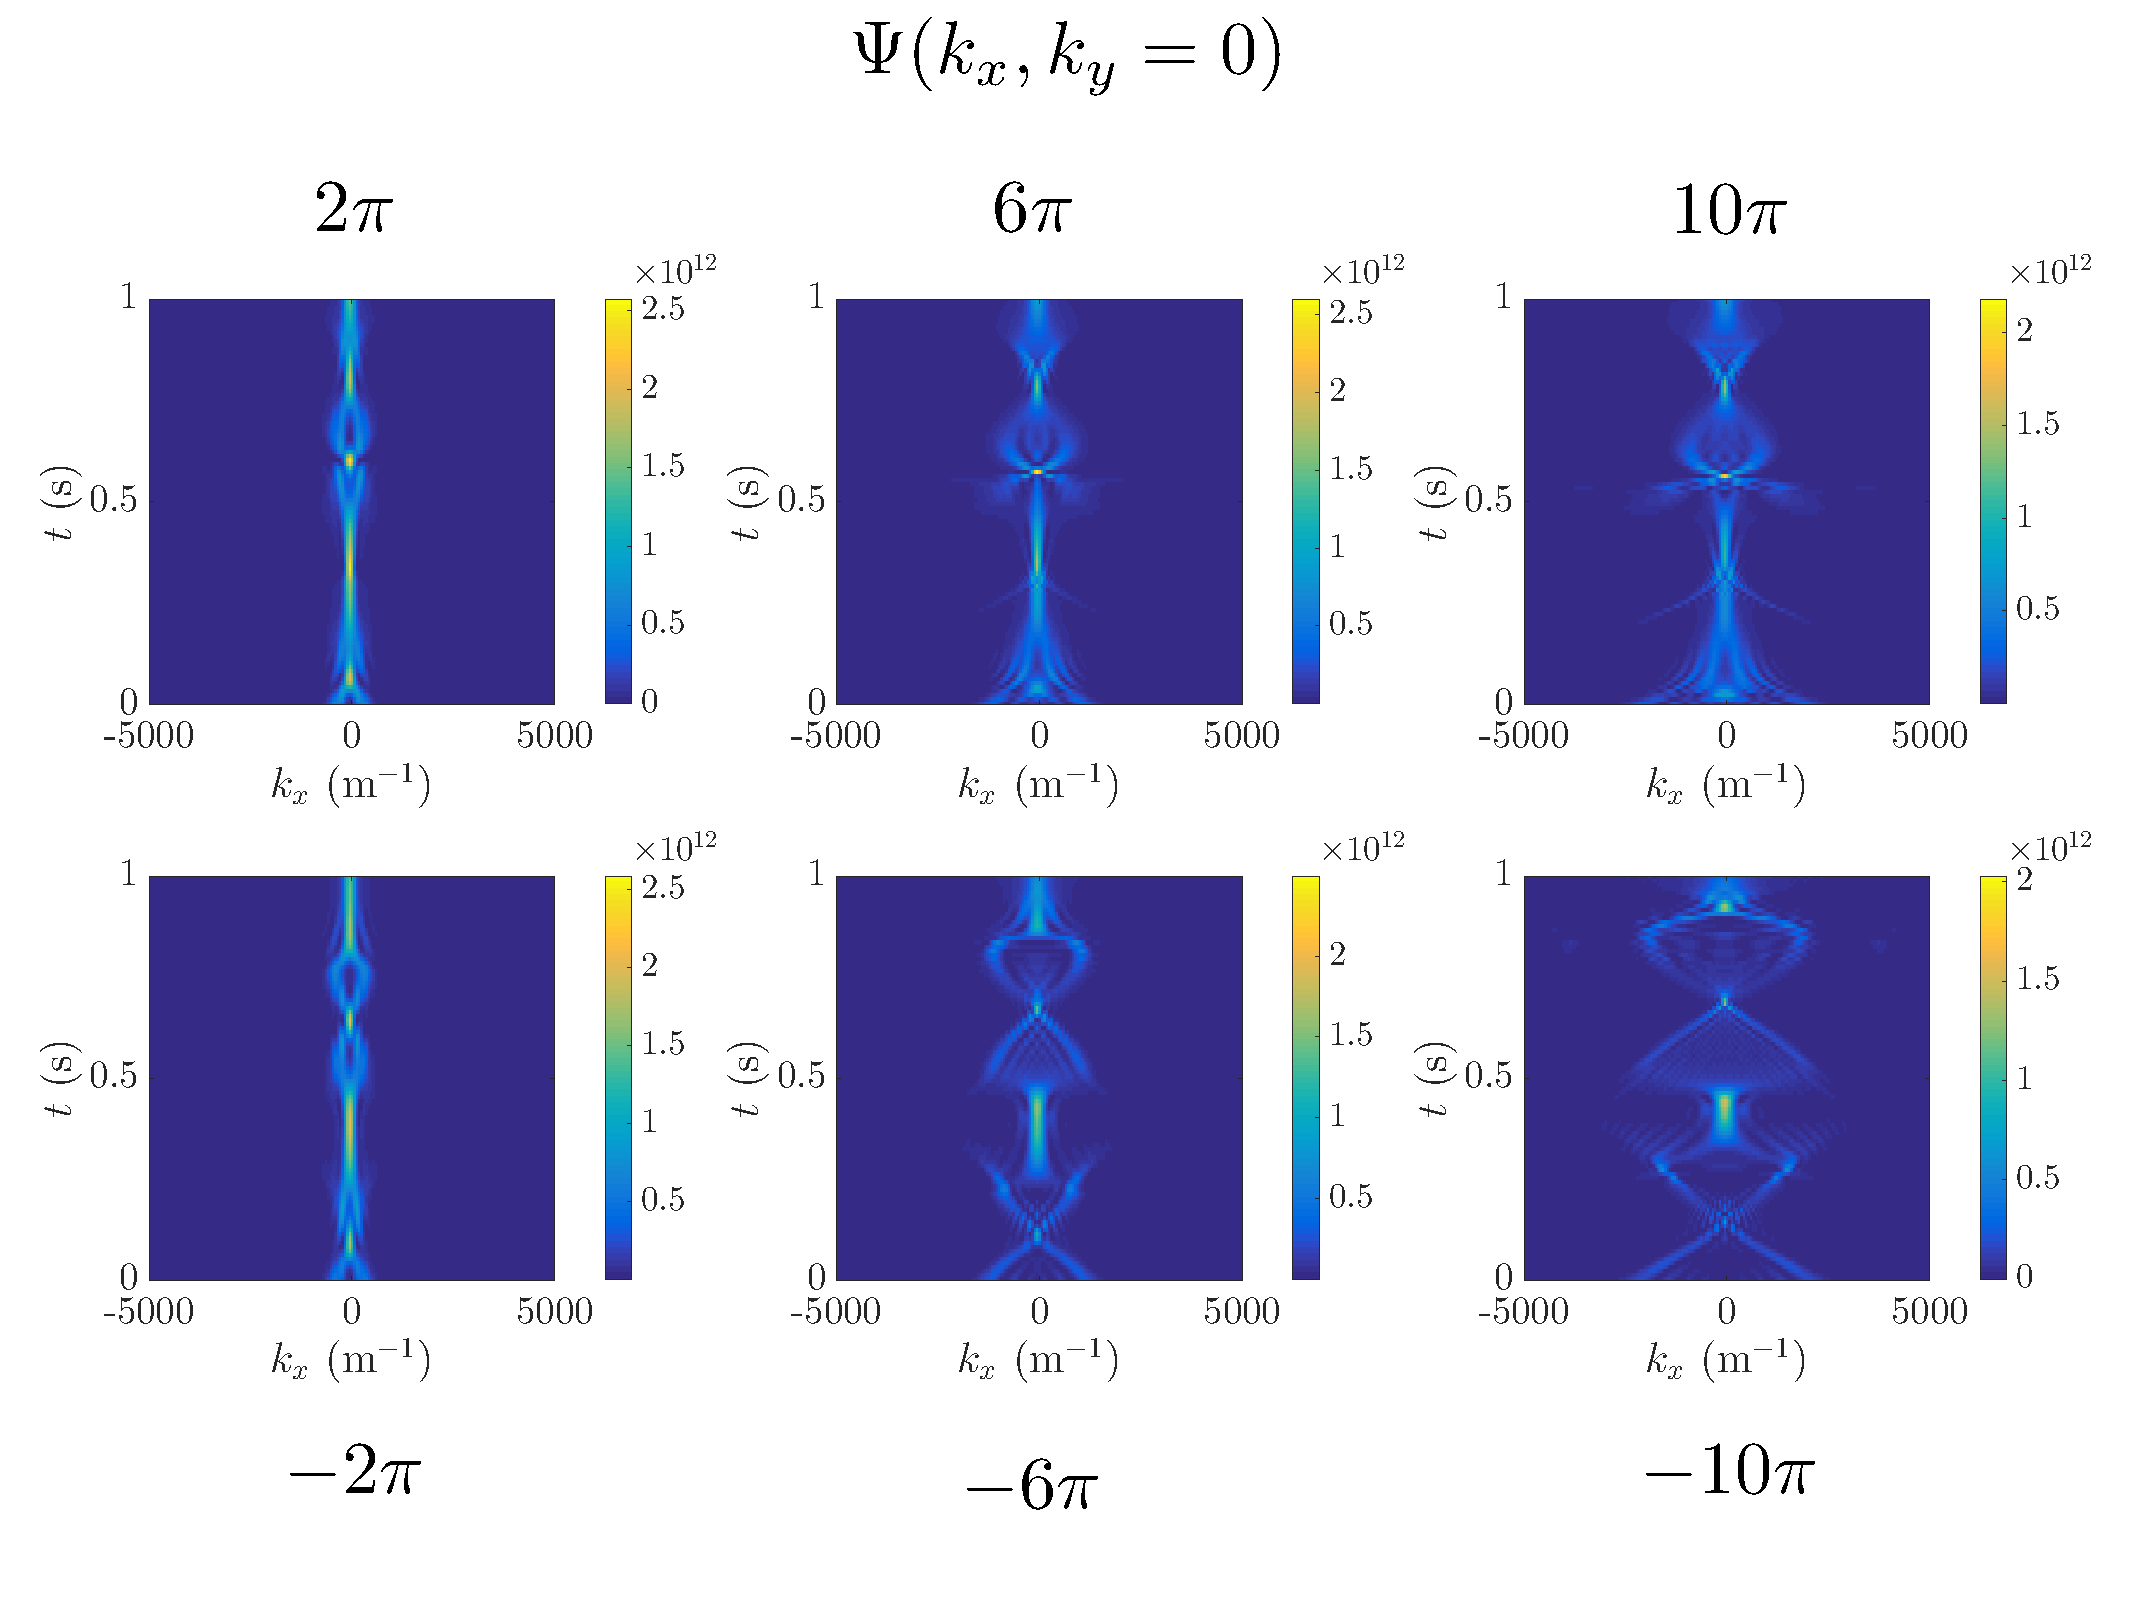
\includegraphics[width=0.95\textwidth]{Images/ch4_vtx/velocity/gaussian_imprint_wfck}    \caption{Gaussian imprint as interferometer}.\label{fig:gaussian_wfc}
\end{figure}


Another potential use of this profile imprinting is for the creation of solitonic vortices, (\textit{svortex}) \cite{}. Svortices are shown to exist in asymmetric 2D condensates, where the harmonic oscillator aspect ratio in the transverse plane has the short axis width approximately twice the healing length \cite{}. This can be achieved by phase imprinting the condensate with a plane-wave directed across a BEC such that the negative gradient of the phase will cause a contraction of the density along one axis onto a centrally located vortex. This can cause the width to approach, and even exceed, the required spatial criterion for observing a svortex. Though this was not investigated thoroughly, the resulting density profiles as shown in Fig.~\ref{fig:svortex} qualitatively matches that of experimentally identified svortices \cite{}. Given the strength of excitation required to allow for this, further analysis would be required in the context of coupling with higher modes and the thermal cloud to determine realism of this model. I will leave this to future work.

\begin{figure}\centering
    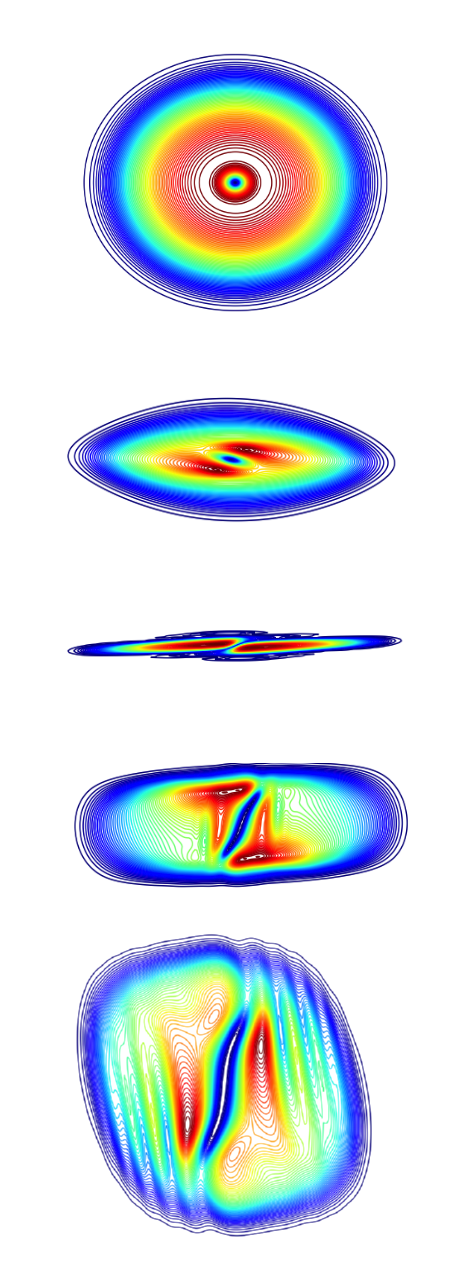
\includegraphics[angle=90,width=0.85\textwidth]{Images/ch4_vtx/velocity/cos_plane_ev}
    \caption{Svortex}.\label{fig:svortex}
\end{figure}

%%%%%%%%%%%%%%%%%%%%%%%%%%%%%%%%%%%%%%%%%%%%%%%%%%%%%%%%%%%%
\subsection{Kinetic energy decomposition}
%%%%%%%%%%%%%%%%%%%%%%%%%%%%%%%%%%%%%%%%%%%%%%%%%%%%%%%%%%%%

To study the effect the above perturbations have on the condensate, I apply a spectral decomposition of the kinetic energy of the condensate into contributions solely from the vortices (incompressible), and those from the phonons (compressible)~\cite{CT:Nore_prl_1997,CT:Nore_pof_1997,CT:Bradley_prx_2012}. For this the wavefunction is first written in terms of amplitude $\sqrt{\rho(\mathbf{r},t)}$ and phase $S(\mathbf{r},t)$ form via a Madelung transform as given by \ref{eqn:madelung}. Making use of the Gross--Pitaevskii energy functional \ref{eqn:functional_kin} gives
\begin{equation}
    E_{\text{kqp}} = \int d\mathbf{r} \left( \frac{\hbar^2}{2m}| \nabla\sqrt{\rho(\mathbf{r},t)} |^2  + \frac{m}{2}|\sqrt{\rho(\mathbf{r},t)}\mathbf{v}(\mathbf{r},t) |^2\right).
\end{equation}
One can decompose this into the quantum pressure (first) and kinetic energy (second) terms. The kinetic energy term can seen as a density-weighted velocity field, $\mathbf{u}(\mathbf{r},t) = \sqrt{\rho(\mathbf{r},t)}\mathbf{v}(\mathbf{r},t)$. This can be further decomposed into the sum of compressible and incompressible terms,
\begin{equation}\label{eqn:kin_en}
    \mathbf{u(r},t) = \mathbf{u}^c(\mathbf{r},t) + \mathbf{u}^i(\mathbf{r},t),
\end{equation}
where $\mathbf{u}^c, \mathbf{u}^i$ are the compressible and incompressible terms respectively. This can be solved for both terms by performing a Helmholtz decomposition on the resulting field, separating terms that are longitudinal ($\mathbf{u}^c$) and transverse ($\mathbf{u}^i$) with
\begin{subequations}\label{eqn:kinterms}
\begin{align}
    \nabla \times \mathbf{u}^c(\mathbf{r},t) = 0, \\
    \nabla \cdot \mathbf{u}^i(\mathbf{r},t) = 0.
\end{align}
\end{subequations}
By introducing the vector potential, $\mathbf{A}$, and scalar potential, $B$, such that
\begin{subequations}
\begin{align}
    \mathbf{u}^c = \nabla B, \\
    \mathbf{u}^i = \nabla \times \mathbf{A}
\end{align}
\end{subequations}
we can rewrite eq.~\ref{eqn:kin_en} as
\begin{align}
    \nabla \times \mathbf{u}(\mathbf{r},t) = -\nabla^2 \mathbf{A}, \\
    \nabla \cdot \mathbf{u}(\mathbf{r},t) = \nabla^2 {B}.
\end{align}

To solve the above equation I begin by seeking a solution for $B$ by performing a spectral decomposition as
\begin{equation}
    B = \displaystyle\sum\limits_{j} \frac{k_j}{|\mathbf{k}|^2}\mathscr{F}[\mathbf{u}],
\end{equation}
where $k_j$ is the $j$-th component in $\mathbf{k}$ space, and $\mathscr{F}$ is the Fourier transform. The resulting solution for $\mathbf{u}^c$ is given by
\begin{equation}
    \mathscr{F}[\mathbf{u}_i^c] = \displaystyle\sum\limits_{j} \frac{k_i k_j}{|\mathbf{k}|^2} \mathscr{F}[\mathbf{u}],
\end{equation}
which after taking note of eq.~\ref{eqn:kin_en} gives
\begin{align}
    \mathscr{F}[\mathbf{u}_i^i] &= \mathscr{F}[\mathbf{u}_i] - \mathscr{F}[\mathbf{u}_i^c]. \\
    &= \displaystyle\sum\limits_{j}\left(\delta_{i,j} - \frac{k_ik_j}{|\mathbf{k}|^2}\right)\mathscr{F}[\mathbf{u}_i]. \nonumber
\end{align}

This decomposition separates the energy contribution from phonons and vortex cores, represented by compressible and incompressible terms respectively~\cite{CT:Horng_pra_2009}. By averaging over binned shells in $\mathbf{k}$-space, the kinetic energy spectra, $E^{c,i}(k)$, are calculated as~\cite{CT:Bradley_prx_2012}
\begin{equation}
	E^{c,i}(k) = \frac{mk}{2}\sum\limits_{j\in\mathbf{r}} \int\limits_{0}^{2\pi}d\phi_k \frac{ |\mathcal{U}_j^{c,i}(\mathbf{k},t) |^2}{s_k},
\end{equation}
where
\begin{equation}
	\mathcal{U}_j^{c,i}(\mathbf{k},t) = \int d^2 \mathbf{r} e^{-i(\mathbf{k}\cdot\mathbf{r})} u_j^{c,i}(\mathbf{r},t).
\end{equation}
The terms $u_j^{c,i}(\mathbf{r},t)$ represent the position-space density-weighted velocity components in the specified shell, where $\phi_k$ is the polar angle, and $s_k$ is the number of values in the chosen shell.
